%! Author = chtompki
%! Date = 1/14/26
\documentclass[10pt]{amsart}
% Default margins are too wide all the way around. I reset them here
\setlength{\hoffset}{-.75in}
\setlength{\textwidth}{6.5in}
\setlength{\voffset}{-.5in}
\setlength{\textheight}{9.0in}
\usepackage{amsmath}
\usepackage{amssymb}
\usepackage{amsthm}
\usepackage{lmodern}
\usepackage{microtype}
\usepackage{enumitem}
\usepackage{setspace}
\usepackage{graphicx}
\usepackage{hyperref}
\usepackage{tikz}
\usetikzlibrary{decorations.markings}
\usepackage{listings}
\usepackage{pgfplots}
\pgfplotsset{compat=1.18}
\usepgfplotslibrary{groupplots}


\newenvironment{solution}
{\begin{proof}[Solution]}
{\end{proof}}

\NewDocumentCommand{\vitem}{v}{%
    \item[\texttt{#1}]%
}

\newcommand{\slopeelement}[3]{%
    \pgfmathsetmacro{\slopeDX}{0.14/sqrt(1+(#3)^2)}%
    \pgfmathsetmacro{\slopeDY}{(#3)*\slopeDX}%
    \pgfmathsetmacro{\slopeXA}{(#1)-\slopeDX}%
    \pgfmathsetmacro{\slopeYA}{(#2)-\slopeDY}%
    \pgfmathsetmacro{\slopeXB}{(#1)+\slopeDX}%
    \pgfmathsetmacro{\slopeYB}{(#2)+\slopeDY}%
    \edef\slopecommand{%
        \noexpand\draw[gray,thin]
        (axis cs:\slopeXA,\slopeYA)
        --
        (axis cs:\slopeXB,\slopeYB);%
    }%
    \slopecommand
}

\title{Dynamical Systems\\Problem Set 4}
\author{Rob Tompkins}
\date{\today}

\begin{document}
    \maketitle
    \date{\today}
    \begin{onehalfspace}
        We begin by noting that all of the files referenced in this document are available at: \\
        \underline{https://github.com/chtompki/MathFall2026/tree/main/DynamicalSystems/ProblemSet4}

        \noindent\textbf{8.1.6}
        Consider the system $\dot{x}=y-2x$, $\dot{y}=\mu+x^2-y$.
        \begin{enumerate}[label=\alph*)]
            \item Sketch the nullclines.
            \item Find and classify the bifurcations that occur as $\mu$ varies.
            \item Sketch the phase portrait as a function of $\mu$.
        \end{enumerate}

        \begin{solution}
\textbf{(a) Nullclines.} Setting each component of the vector field equal to zero gives
\[
    \dot{x}=0:\quad y=2x,
    \qquad
    \dot{y}=0:\quad y=x^2+\mu.
\]
Thus the nullclines are a fixed straight line and an upward-opening parabola that moves vertically with $\mu$. The direction of the flow is determined by
\[
\begin{array}{c|cc}
 & \text{condition} & \text{direction}\\ \hline
\dot{x}>0 & y>2x & \text{right}\\
\dot{x}<0 & y<2x & \text{left}\\
\dot{y}>0 & y<x^2+\mu & \text{up}\\
\dot{y}<0 & y>x^2+\mu & \text{down}
\end{array}
\]
The nullclines intersect when
\[
    x^2-2x+\mu=(x-1)^2+\mu-1=0.
\]
For $\mu<1$, the two equilibria are
\[
    P_-=\bigl(1-\sqrt{1-\mu},\,2-2\sqrt{1-\mu}\bigr),\qquad P_+=\bigl(1+\sqrt{1-\mu},\,2+2\sqrt{1-\mu}\bigr).
\]
At $\mu=1$ they coincide at $(1,2)$, where the nullclines are tangent; for $\mu>1$ there are no equilibria.

\medskip
\noindent\textbf{Nullcline sketches and equilibrium stability.}
The following sketches use $\mu=0,1,2$ as representatives of the three cases. Blue denotes $y=2x$ and red denotes $y=x^2+\mu$. For $\mu\leq1$, solid portions on the $x<1$ side indicate the attracting equilibrium branch, and dotted portions on the $x>1$ side indicate the saddle branch or the repelling side of the saddle-node. These line styles are visual guides to the classification at the intersections: points elsewhere on a nullcline are not equilibria and do not themselves have a stability classification. In particular, the dotted branch at the saddle does not mean that both eigen-directions are unstable.

\begin{center}
\begin{tikzpicture}[x=1.12cm,y=0.61cm,>=stealth,font=\small]
\path[use as bounding box] (-1,-1.4) rectangle (3.6,8.4);
\draw[->] (-.65,0)--(3.25,0) node[right] {$x$};
\draw[->] (0,-.65)--(0,6.9) node[left] {$y$};
\node at (1.25,7.7) {$\mu<1$ (shown: $\mu=0$)};
\draw (1,.08)--(1,-.08) node[below] {$1$};
\draw (2,.08)--(2,-.08) node[below] {$2$};
\draw (.06,2)--(-.06,2) node[left] {$2$};
\draw (.06,4)--(-.06,4) node[left] {$4$};
\begin{scope}
\clip (-.65,-.65) rectangle (3.05,6.6);
\draw[blue,thick,domain=-.65:1,samples=70] plot (\x,{2*\x});
\draw[blue,thick,densely dotted,domain=1:3.05,samples=70] plot (\x,{2*\x});
\draw[red,thick,domain=-.65:1,samples=70] plot (\x,{\x*\x+0});
\draw[red,thick,densely dotted,domain=1:3.05,samples=70] plot (\x,{\x*\x+0});
\end{scope}
\fill (0,0) circle (2.5pt);
\node[fill=white,inner sep=1pt] at (.8,.65) {stable};
\draw[fill=white,thick] (2,4) circle (2.5pt);
\node[anchor=west,fill=white,inner sep=1pt] at (2.12,3.8) {saddle};
\node[align=center] at (1.2,-1.1) {two equilibria};
\end{tikzpicture}
\hfill
\begin{tikzpicture}[x=1.12cm,y=0.61cm,>=stealth,font=\small]
\path[use as bounding box] (-1,-1.4) rectangle (3.6,8.4);
\draw[->] (-.65,0)--(3.25,0) node[right] {$x$};
\draw[->] (0,-.65)--(0,6.9) node[left] {$y$};
\node at (1.25,7.7) {$\mu=1$};
\draw (1,.08)--(1,-.08) node[below] {$1$};
\draw (2,.08)--(2,-.08) node[below] {$2$};
\draw (.06,2)--(-.06,2) node[left] {$2$};
\draw (.06,4)--(-.06,4) node[left] {$4$};
\begin{scope}
\clip (-.65,-.65) rectangle (3.05,6.6);
\draw[blue,thick,domain=-.65:1,samples=70] plot (\x,{2*\x});
\draw[blue,thick,densely dotted,domain=1:3.05,samples=70] plot (\x,{2*\x});
\draw[red,thick,domain=-.65:1,samples=70] plot (\x,{\x*\x+1});
\draw[red,thick,densely dotted,domain=1:3.05,samples=70] plot (\x,{\x*\x+1});
\end{scope}
\draw[fill=white,thick] (1,2) circle (2.5pt);
\begin{scope}\clip (1,2) circle (2.5pt);
\fill (.8,1.8) rectangle (1,2.2);\end{scope}
\node[anchor=west,fill=white,inner sep=1pt] at (1.15,1.7) {saddle-node};
\node[align=center] at (1.2,-1.1) {one-sided attraction};
\end{tikzpicture}
\hfill
\begin{tikzpicture}[x=1.12cm,y=0.61cm,>=stealth,font=\small]
\path[use as bounding box] (-1,-1.4) rectangle (3.6,8.4);
\draw[->] (-.65,0)--(3.25,0) node[right] {$x$};
\draw[->] (0,-.65)--(0,6.9) node[left] {$y$};
\node at (1.25,7.7) {$\mu>1$ (shown: $\mu=2$)};
\draw (1,.08)--(1,-.08) node[below] {$1$};
\draw (2,.08)--(2,-.08) node[below] {$2$};
\draw (.06,2)--(-.06,2) node[left] {$2$};
\draw (.06,4)--(-.06,4) node[left] {$4$};
\begin{scope}
\clip (-.65,-.65) rectangle (3.05,6.6);
\draw[blue!65,thin,domain=-.65:3.05,samples=80] plot (\x,{2*\x});
\draw[red!65,thin,domain=-.65:3.05,samples=80] plot (\x,{\x*\x+2});
\end{scope}
\node[align=center,fill=white,inner sep=2pt] at (1.5,1.5) {no intersections};
\node[align=center] at (1.2,-1.1) {no equilibrium stability};
\end{tikzpicture}
\end{center}
At $\mu=1$, ``one-sided attraction'' refers to the center-manifold dynamics: the equilibrium attracts from the left and repels to the right, while the transverse direction is stable. It is therefore not a stable equilibrium in the Lyapunov sense. For $\mu>1$, the curves are shown thin because there is no equilibrium to classify; calling either nullcline stable or unstable would be misleading.


\medskip
\textbf{(b) Jacobian and stability.} The Jacobian is
\[
    J(x,y)=
    \begin{pmatrix}-2&1\\2x&-1\end{pmatrix}.
\]
At the two equilibria, substitute $x=1\pm\sqrt{1-\mu}$ directly into the Jacobian:
\[
    J(P_\pm)=\begin{pmatrix}
        -2&1\\2\pm2\sqrt{1-\mu}&-1
    \end{pmatrix}.
\]
Their traces, determinants, and characteristic polynomials are
\[
    \tau_\pm=-3,\qquad \Delta_\pm=-\bigl(\pm2\sqrt{1-\mu}\bigr),
\]
\[
    \det(\lambda I-J(P_\pm))
       =\lambda^2+3\lambda-\bigl(\pm2\sqrt{1-\mu}\bigr).
\]
Here the upper sign corresponds to $P_+$ and the lower sign to $P_-$. We examine the two branches separately below.
At the lower equilibrium $P_-$,
\[
    J_- =\begin{pmatrix}-2&1\\2-2\sqrt{1-\mu}&-1\end{pmatrix},
    \qquad \Delta_-=2\sqrt{1-\mu}>0.
\]
\[
    \lambda_{1,2}^{(-)}=\frac{-3\pm\sqrt{9-8\sqrt{1-\mu}}}2.
\]
Since the trace is negative and the determinant is positive, both eigenvalues have negative real parts. Hence $P_-$ is asymptotically stable for every $\mu<1$. More precisely,
\[
\begin{array}{c|c|c}
\text{parameter range}&\text{eigenvalues at }P_-&\text{classification}\\ \hline
\mu<-17/64 & \text{complex, real part }-3/2 & \text{stable spiral}\\
\mu=-17/64 & \lambda_1=\lambda_2=-3/2 & \text{improper stable node}\\
-17/64<\mu<1 & \text{distinct, real, negative} & \text{stable node}
\end{array}
\]
Indeed, $9-8\sqrt{1-\mu}=0$ gives $\sqrt{1-\mu}=9/8$ and $\mu=1-(9/8)^2=-17/64$. At this value $J_-\ne-\tfrac32 I$, so the repeated eigenvalue has only one independent eigenvector. This spiral-to-node transition does not change stability and is not a bifurcation of the local topological phase portrait.

At the upper equilibrium $P_+$,
\[
    J_+=\begin{pmatrix}-2&1\\2+2\sqrt{1-\mu}&-1\end{pmatrix},
    \qquad \Delta_+=-2\sqrt{1-\mu}<0.
\]
\[
    \lambda_{1,2}^{(+)}=\frac{-3\pm\sqrt{9+8\sqrt{1-\mu}}}2.
\]
One eigenvalue is positive and one is negative, so $P_+$ is always an unstable saddle.

At $\mu=1$,
\[
    J(1,2)=\begin{pmatrix}-2&1\\2&-1\end{pmatrix},
    \qquad \lambda_1=0,\quad\lambda_2=-3.
\]
Linearization alone cannot classify the zero-eigenvalue direction. Set
\[
    u=x-1,\qquad w=y-2x,\qquad \delta=\mu-1.
\]
Then the system becomes exactly
\[
    \dot{u}=w,\qquad \dot{w}=\delta+u^2-3w.
\]
At $\delta=0$, a center manifold $w=h(u)$ satisfies
\[
    h'(u)h(u)=u^2-3h(u).
\]
Writing $h(u)=a u^2+O(u^3)$ and comparing quadratic terms gives $a=1/3$. Thus the reduced equation is
\[
    \dot{u}=\tfrac13u^2+O(u^3).
\]
The equilibrium attracts along the center manifold from $u<0$ and repels toward $u>0$, while the transverse direction is attracting. In particular, it is not Lyapunov stable. Including the parameter gives the local saddle-node form
\[
    \dot{u}=\tfrac13(\delta+u^2)
       +O\bigl(|u|^3+|\delta u|+\delta^2\bigr).
\]
Therefore a stable equilibrium and a saddle collide and disappear at
\[
    \mu_c=1\quad\text{(saddle-node bifurcation).}
\]
No Hopf bifurcation is possible because the trace is always $-3$. Also,
$\partial\dot{x}/\partial x+\partial\dot{y}/\partial y=-3$ everywhere, so Bendixson's criterion excludes periodic orbits in the plane.

\begin{center}
\begin{tikzpicture}
\begin{axis}[width=9cm,height=5cm,axis lines=middle,
    xmin=-2,xmax=1.6,ymin=-0.9,ymax=2.9,
    xlabel={$\mu$},ylabel={$1\pm\sqrt{1-\mu}$},
    xtick={-1,0,1},ytick={0,1,2},
    clip=false,legend columns=2,
    legend style={at={(0.5,-0.2)},anchor=north,font=\small}]
    \addplot[blue,thick,domain=-0.7:1,samples=100,variable=\t]
        ({1-(t-1)^2},{t});
    \addlegendentry{attracting equilibrium}
    \addplot[red,dashed,thick,domain=1:2.7,samples=100,variable=\t]
        ({1-(t-1)^2},{t});
    \addlegendentry{saddle}
    \addplot[only marks,mark=*,black] coordinates {(1,1)};
    \node[anchor=west,font=\small] at (axis cs:1.05,1.3) {saddle-node};
\end{axis}
\end{tikzpicture}
\end{center}

\textbf{(c) Phase portraits.} The plots below show representative cases on either side of $\mu=1$ and at the bifurcation. Blue solid curves are $\dot{x}=0$, red dashed curves are $\dot{y}=0$, and gray arrows give the flow direction. Black curves are numerically integrated trajectories; their arrows indicate increasing time. At the saddle, the green curves show its stable and unstable separatrices. A filled point marks the attractor, an open point the saddle, and a half-filled point the saddle-node.

\begin{center}
\begin{tikzpicture}[x=1.12cm,y=0.61cm,>=stealth]
\path[use as bounding box] (-1,-1.6) rectangle (3.55,7.6);
\draw[->] (-.8,0)--(3.35,0) node[right] {$x$};
\draw[->] (0,-1.1)--(0,7) node[left] {$y$};
\node[font=\small] at (1.25,7.5) {$\mu=-1$: spiral and saddle};
\begin{scope}
\clip (-.8,-1) rectangle (3.1,6.5);
\draw[->,gray!55,thin] (-0.6574,-0.7069)--(-0.5426,-0.6931);
\draw[->,gray!55,thin] (-0.1168,-0.6599)--(-0.2232,-0.7401);
\draw[->,gray!55,thin] (0.3172,-0.6891)--(0.2028,-0.7109);
\draw[->,gray!55,thin] (0.7474,-0.7049)--(0.6326,-0.6951);
\draw[->,gray!55,thin] (1.1766,-0.7184)--(1.0634,-0.6816);
\draw[->,gray!55,thin] (1.6051,-0.7305)--(1.4949,-0.6695);
\draw[->,gray!55,thin] (2.0330,-0.7411)--(1.9270,-0.6589);
\draw[->,gray!55,thin] (2.4605,-0.7504)--(2.3595,-0.6496);
\draw[->,gray!55,thin] (2.8879,-0.7583)--(2.7921,-0.6417);
\draw[->,gray!55,thin] (-0.6555,-0.0523)--(-0.5445,-0.1077);
\draw[->,gray!55,thin] (-0.1972,0.0131)--(-0.1428,-0.1731);
\draw[->,gray!55,thin] (0.3055,-0.0154)--(0.2145,-0.1446);
\draw[->,gray!55,thin] (0.7467,-0.0628)--(0.6333,-0.0972);
\draw[->,gray!55,thin] (1.1773,-0.0883)--(1.0627,-0.0717);
\draw[->,gray!55,thin] (1.6057,-0.1060)--(1.4943,-0.0540);
\draw[->,gray!55,thin] (2.0333,-0.1196)--(1.9267,-0.0404);
\draw[->,gray!55,thin] (2.4605,-0.1304)--(2.3595,-0.0296);
\draw[->,gray!55,thin] (2.8876,-0.1391)--(2.7924,-0.0209);
\draw[->,gray!55,thin] (-0.6539,0.5766)--(-0.5461,0.5034);
\draw[->,gray!55,thin] (-0.2120,0.6121)--(-0.1280,0.4679);
\draw[->,gray!55,thin] (0.2586,0.6455)--(0.2614,0.4345);
\draw[->,gray!55,thin] (0.7373,0.5999)--(0.6427,0.4801);
\draw[->,gray!55,thin] (1.1773,0.5496)--(1.0627,0.5304);
\draw[->,gray!55,thin] (1.6066,0.5209)--(1.4934,0.5591);
\draw[->,gray!55,thin] (2.0338,0.5026)--(1.9262,0.5774);
\draw[->,gray!55,thin] (2.4605,0.4896)--(2.3595,0.5904);
\draw[->,gray!55,thin] (2.8873,0.4800)--(2.7927,0.6000);
\draw[->,gray!55,thin] (-0.6531,1.2005)--(-0.5469,1.1195);
\draw[->,gray!55,thin] (-0.2155,1.2246)--(-0.1245,1.0954);
\draw[->,gray!55,thin] (0.2318,1.2521)--(0.2882,1.0679);
\draw[->,gray!55,thin] (0.7034,1.2627)--(0.6766,1.0573);
\draw[->,gray!55,thin] (1.1723,1.2039)--(1.0677,1.1161);
\draw[->,gray!55,thin] (1.6074,1.1528)--(1.4926,1.1672);
\draw[->,gray!55,thin] (2.0344,1.1258)--(1.9256,1.1942);
\draw[->,gray!55,thin] (2.4605,1.1096)--(2.3595,1.2104);
\draw[->,gray!55,thin] (2.8868,1.0988)--(2.7932,1.2212);
\draw[->,gray!55,thin] (-0.6526,1.8227)--(-0.5474,1.7373);
\draw[->,gray!55,thin] (-0.2170,1.8409)--(-0.1230,1.7191);
\draw[->,gray!55,thin] (0.2227,1.8603)--(0.2973,1.6997);
\draw[->,gray!55,thin] (0.6725,1.8806)--(0.7075,1.6794);
\draw[->,gray!55,thin] (1.1478,1.8724)--(1.0922,1.6876);
\draw[->,gray!55,thin] (1.6068,1.7962)--(1.4932,1.7638);
\draw[->,gray!55,thin] (2.0353,1.7511)--(1.9247,1.8089);
\draw[->,gray!55,thin] (2.4605,1.7297)--(2.3595,1.8303);
\draw[->,gray!55,thin] (2.8863,1.7173)--(2.7937,1.8427);
\draw[->,gray!55,thin] (-0.6522,2.4441)--(-0.5478,2.3559);
\draw[->,gray!55,thin] (-0.2178,2.4588)--(-0.1222,2.3412);
\draw[->,gray!55,thin] (0.2186,2.4733)--(0.3014,2.3267);
\draw[->,gray!55,thin] (0.6590,2.4889)--(0.7210,2.3111);
\draw[->,gray!55,thin] (1.1122,2.5046)--(1.1278,2.2954);
\draw[->,gray!55,thin] (1.5954,2.4647)--(1.5046,2.3353);
\draw[->,gray!55,thin] (2.0366,2.3811)--(1.9234,2.4189);
\draw[->,gray!55,thin] (2.4606,2.3497)--(2.3594,2.4503);
\draw[->,gray!55,thin] (2.8855,2.3353)--(2.7945,2.4647);
\draw[->,gray!55,thin] (-0.6520,3.0651)--(-0.5480,2.9749);
\draw[->,gray!55,thin] (-0.2183,3.0773)--(-0.1217,2.9627);
\draw[->,gray!55,thin] (0.2164,3.0889)--(0.3036,2.9511);
\draw[->,gray!55,thin] (0.6528,3.1005)--(0.7272,2.9395);
\draw[->,gray!55,thin] (1.0936,3.1137)--(1.1464,2.9263);
\draw[->,gray!55,thin] (1.5552,3.1251)--(1.5448,2.9149);
\draw[->,gray!55,thin] (2.0374,3.0261)--(1.9226,3.0139);
\draw[->,gray!55,thin] (2.4606,2.9698)--(2.3594,3.0702);
\draw[->,gray!55,thin] (2.8843,2.9527)--(2.7957,3.0873);
\draw[->,gray!55,thin] (-0.6518,3.6858)--(-0.5482,3.5942);
\draw[->,gray!55,thin] (-0.2186,3.6963)--(-0.1214,3.5837);
\draw[->,gray!55,thin] (0.2151,3.7059)--(0.3049,3.5741);
\draw[->,gray!55,thin] (0.6494,3.7148)--(0.7306,3.5652);
\draw[->,gray!55,thin] (1.0852,3.7241)--(1.1548,3.5559);
\draw[->,gray!55,thin] (1.5267,3.7365)--(1.5733,3.5435);
\draw[->,gray!55,thin] (2.0164,3.7218)--(1.9436,3.5582);
\draw[->,gray!55,thin] (2.4606,3.5899)--(2.3594,3.6901);
\draw[->,gray!55,thin] (2.8824,3.5687)--(2.7976,3.7113);
\draw[->,gray!55,thin] (-0.6517,4.3064)--(-0.5483,4.2136);
\draw[->,gray!55,thin] (-0.2189,4.3156)--(-0.1211,4.2044);
\draw[->,gray!55,thin] (0.2141,4.3237)--(0.3059,4.1963);
\draw[->,gray!55,thin] (0.6474,4.3308)--(0.7326,4.1892);
\draw[->,gray!55,thin] (1.0809,4.3375)--(1.1591,4.1825);
\draw[->,gray!55,thin] (1.5156,4.3446)--(1.5844,4.1754);
\draw[->,gray!55,thin] (1.9581,4.3576)--(2.0019,4.1624);
\draw[->,gray!55,thin] (2.4607,4.2103)--(2.3593,4.3097);
\draw[->,gray!55,thin] (2.8791,4.1827)--(2.8009,4.3373);
\draw[->,gray!55,thin] (-0.6515,4.9268)--(-0.5485,4.8332);
\draw[->,gray!55,thin] (-0.2191,4.9350)--(-0.1209,4.8250);
\draw[->,gray!55,thin] (0.2135,4.9420)--(0.3065,4.8180);
\draw[->,gray!55,thin] (0.6460,4.9479)--(0.7340,4.8121);
\draw[->,gray!55,thin] (1.0784,4.9529)--(1.1616,4.8071);
\draw[->,gray!55,thin] (1.5106,4.9569)--(1.5894,4.8031);
\draw[->,gray!55,thin] (1.9425,4.9600)--(2.0175,4.8000);
\draw[->,gray!55,thin] (2.8721,4.7924)--(2.8079,4.9676);
\draw[->,gray!55,thin] (-0.6514,5.5471)--(-0.5486,5.4529);
\draw[->,gray!55,thin] (-0.2192,5.5545)--(-0.1208,5.4455);
\draw[->,gray!55,thin] (0.2130,5.5607)--(0.3070,5.4393);
\draw[->,gray!55,thin] (0.6450,5.5658)--(0.7350,5.4342);
\draw[->,gray!55,thin] (1.0768,5.5696)--(1.1632,5.4304);
\draw[->,gray!55,thin] (1.5079,5.5719)--(1.5921,5.4281);
\draw[->,gray!55,thin] (1.9375,5.5712)--(2.0225,5.4288);
\draw[->,gray!55,thin] (2.3597,5.5512)--(2.4603,5.4488);
\draw[->,gray!55,thin] (2.8519,5.3967)--(2.8281,5.6033);
\draw[->,gray!55,thin] (-0.6514,6.1674)--(-0.5486,6.0726);
\draw[->,gray!55,thin] (-0.2194,6.1742)--(-0.1206,6.0658);
\draw[->,gray!55,thin] (0.2126,6.1797)--(0.3074,6.0603);
\draw[->,gray!55,thin] (0.6443,6.1841)--(0.7357,6.0559);
\draw[->,gray!55,thin] (1.0756,6.1871)--(1.1644,6.0529);
\draw[->,gray!55,thin] (1.5062,6.1884)--(1.5938,6.0516);
\draw[->,gray!55,thin] (1.9352,6.1863)--(2.0248,6.0537);
\draw[->,gray!55,thin] (2.3596,6.1709)--(2.4604,6.0691);
\draw[->,gray!55,thin] (2.8027,6.0397)--(2.8773,6.2003);
\draw[blue,thick,domain=-.8:3.1,samples=80] plot (\x,{2*\x});
\draw[red,dashed,thick,domain=-.8:3.1,samples=80] plot (\x,{\x*\x+-1});
\draw[black!80,thin,postaction={decorate},decoration={markings,mark=at position 0.42 with {\arrow{stealth}}}] plot coordinates {(-0.1000,-0.8000) (-0.1071,-0.8023) (-0.1470,-0.8149) (-0.1823,-0.8258) (-0.2136,-0.8352) (-0.2412,-0.8430) (-0.2656,-0.8494) (-0.2871,-0.8546) (-0.3061,-0.8586) (-0.3227,-0.8615) (-0.3373,-0.8635) (-0.3500,-0.8648) (-0.3611,-0.8654) (-0.3707,-0.8654) (-0.3790,-0.8650) (-0.3861,-0.8642) (-0.3923,-0.8631) (-0.3975,-0.8618) (-0.4019,-0.8603) (-0.4057,-0.8587) (-0.4088,-0.8570) (-0.4114,-0.8552) (-0.4135,-0.8535) (-0.4152,-0.8517) (-0.4166,-0.8500) (-0.4176,-0.8483) (-0.4185,-0.8467) (-0.4191,-0.8452) (-0.4195,-0.8437) (-0.4198,-0.8424) (-0.4199,-0.8411) (-0.4199,-0.8398) (-0.4199,-0.8387) (-0.4198,-0.8377) (-0.4196,-0.8367) (-0.4194,-0.8358) (-0.4192,-0.8350) (-0.4189,-0.8343) (-0.4187,-0.8336) (-0.4184,-0.8330) (-0.4181,-0.8325) (-0.4179,-0.8320) (-0.4176,-0.8315) (-0.4173,-0.8311) (-0.4171,-0.8307) (-0.4168,-0.8304) (-0.4166,-0.8301) (-0.4164,-0.8299) (-0.4162,-0.8297)};
\draw[black!80,thin,postaction={decorate},decoration={markings,mark=at position 0.42 with {\arrow{stealth}}}] plot coordinates {(-0.6500,-0.4000) (-0.6393,-0.4022) (-0.5811,-0.4179) (-0.5318,-0.4369) (-0.4905,-0.4579) (-0.4562,-0.4801) (-0.4280,-0.5027) (-0.4051,-0.5252) (-0.3867,-0.5473) (-0.3723,-0.5688) (-0.3612,-0.5894) (-0.3530,-0.6091) (-0.3471,-0.6277) (-0.3433,-0.6453) (-0.3411,-0.6618) (-0.3403,-0.6773) (-0.3405,-0.6916) (-0.3417,-0.7050) (-0.3436,-0.7173) (-0.3460,-0.7287) (-0.3488,-0.7392) (-0.3519,-0.7488) (-0.3553,-0.7575) (-0.3587,-0.7655) (-0.3622,-0.7728) (-0.3656,-0.7794) (-0.3691,-0.7853) (-0.3724,-0.7907) (-0.3757,-0.7955) (-0.3788,-0.7998) (-0.3817,-0.8037) (-0.3846,-0.8071) (-0.3872,-0.8102) (-0.3897,-0.8129) (-0.3920,-0.8153) (-0.3942,-0.8174) (-0.3962,-0.8192) (-0.3981,-0.8208) (-0.3998,-0.8222) (-0.4013,-0.8234) (-0.4028,-0.8244) (-0.4041,-0.8253) (-0.4052,-0.8261) (-0.4063,-0.8267) (-0.4073,-0.8273) (-0.4081,-0.8277) (-0.4089,-0.8281) (-0.4096,-0.8284) (-0.4102,-0.8286) (-0.4108,-0.8288) (-0.4113,-0.8290) (-0.4117,-0.8291) (-0.4121,-0.8292) (-0.4124,-0.8293)};
\draw[black!80,thin,postaction={decorate},decoration={markings,mark=at position 0.42 with {\arrow{stealth}}}] plot coordinates {(-0.6000,2.4000) (-0.5575,2.3634) (-0.3318,2.1435) (-0.1510,1.9292) (-0.0084,1.7262) (0.1019,1.5371) (0.1852,1.3624) (0.2461,1.2016) (0.2885,1.0537) (0.3158,0.9174) (0.3306,0.7915) (0.3352,0.6748) (0.3318,0.5662) (0.3217,0.4648) (0.3064,0.3699) (0.2871,0.2809) (0.2645,0.1972) (0.2395,0.1184) (0.2128,0.0443) (0.1848,-0.0255) (0.1560,-0.0912) (0.1268,-0.1529) (0.0976,-0.2109) (0.0684,-0.2652) (0.0397,-0.3161) (0.0116,-0.3635) (-0.0159,-0.4077) (-0.0425,-0.4488) (-0.0683,-0.4869) (-0.0930,-0.5221) (-0.1166,-0.5545) (-0.1392,-0.5843) (-0.1607,-0.6116) (-0.1810,-0.6366) (-0.2002,-0.6593) (-0.2183,-0.6799) (-0.2353,-0.6986) (-0.2511,-0.7154) (-0.2660,-0.7305) (-0.2797,-0.7440) (-0.2925,-0.7561) (-0.3044,-0.7669) (-0.3153,-0.7764) (-0.3254,-0.7848) (-0.3346,-0.7922) (-0.3431,-0.7986) (-0.3508,-0.8042) (-0.3579,-0.8091) (-0.3643,-0.8133) (-0.3701,-0.8169) (-0.3754,-0.8200) (-0.3801,-0.8226) (-0.3844,-0.8247) (-0.3882,-0.8265) (-0.3916,-0.8280) (-0.3946,-0.8292) (-0.3974,-0.8302) (-0.3998,-0.8310) (-0.4019,-0.8315) (-0.4038,-0.8320) (-0.4054,-0.8323) (-0.4069,-0.8325) (-0.4081,-0.8326) (-0.4092,-0.8326) (-0.4102,-0.8326) (-0.4110,-0.8325) (-0.4117,-0.8324) (-0.4123,-0.8322) (-0.4128,-0.8321) (-0.4132,-0.8319) (-0.4136,-0.8317) (-0.4139,-0.8315) (-0.4141,-0.8313)};
\draw[black!80,thin,postaction={decorate},decoration={markings,mark=at position 0.42 with {\arrow{stealth}}}] plot coordinates {(0.3000,4.8000) (0.3494,4.7321) (0.6065,4.3506) (0.8051,4.0143) (0.9560,3.7205) (1.0683,3.4643) (1.1494,3.2400) (1.2056,3.0422) (1.2418,2.8657) (1.2618,2.7063) (1.2690,2.5602) (1.2658,2.4246) (1.2542,2.2971) (1.2358,2.1758) (1.2120,2.0593) (1.1836,1.9465) (1.1516,1.8365) (1.1166,1.7288) (1.0791,1.6230) (1.0397,1.5187) (0.9985,1.4159) (0.9561,1.3144) (0.9125,1.2143) (0.8682,1.1155) (0.8232,1.0182) (0.7778,0.9225) (0.7321,0.8285) (0.6863,0.7364) (0.6405,0.6464) (0.5949,0.5585) (0.5497,0.4730) (0.5048,0.3899) (0.4605,0.3095) (0.4168,0.2319) (0.3739,0.1572) (0.3318,0.0854) (0.2906,0.0168) (0.2505,-0.0488) (0.2115,-0.1112) (0.1736,-0.1703) (0.1370,-0.2263) (0.1016,-0.2791) (0.0675,-0.3286) (0.0348,-0.3751) (0.0035,-0.4185) (-0.0264,-0.4589) (-0.0550,-0.4963) (-0.0821,-0.5310) (-0.1078,-0.5629) (-0.1321,-0.5923) (-0.1550,-0.6192) (-0.1766,-0.6437) (-0.1969,-0.6660) (-0.2158,-0.6863) (-0.2335,-0.7045) (-0.2500,-0.7210) (-0.2654,-0.7358) (-0.2796,-0.7489) (-0.2927,-0.7607) (-0.3048,-0.7711) (-0.3160,-0.7803) (-0.3262,-0.7884) (-0.3356,-0.7955) (-0.3441,-0.8017) (-0.3519,-0.8070) (-0.3590,-0.8116) (-0.3654,-0.8156) (-0.3712,-0.8190) (-0.3765,-0.8219) (-0.3812,-0.8243) (-0.3854,-0.8263) (-0.3892,-0.8279) (-0.3925,-0.8292) (-0.3955,-0.8303) (-0.3982,-0.8312) (-0.4006,-0.8318) (-0.4026,-0.8323) (-0.4045,-0.8326) (-0.4061,-0.8328) (-0.4074,-0.8330) (-0.4087,-0.8330) (-0.4097,-0.8330) (-0.4106,-0.8329) (-0.4114,-0.8328) (-0.4121,-0.8326) (-0.4126,-0.8324) (-0.4131,-0.8322) (-0.4135,-0.8320) (-0.4138,-0.8318) (-0.4141,-0.8316) (-0.4143,-0.8313)};
\draw[black!80,thin,postaction={decorate},decoration={markings,mark=at position 0.42 with {\arrow{stealth}}}] plot coordinates {(1.4000,0.1000) (1.3680,0.1097) (1.1934,0.1462) (1.0435,0.1531) (0.9135,0.1393) (0.7994,0.1110) (0.6983,0.0727) (0.6080,0.0277) (0.5267,-0.0214) (0.4529,-0.0727) (0.3855,-0.1250) (0.3236,-0.1770) (0.2666,-0.2282) (0.2138,-0.2778) (0.1649,-0.3255) (0.1193,-0.3709) (0.0770,-0.4140) (0.0375,-0.4544) (0.0007,-0.4923) (-0.0337,-0.5275) (-0.0656,-0.5602) (-0.0955,-0.5903) (-0.1232,-0.6179) (-0.1490,-0.6432) (-0.1729,-0.6661) (-0.1951,-0.6870) (-0.2157,-0.7058) (-0.2347,-0.7227) (-0.2522,-0.7378) (-0.2683,-0.7513) (-0.2831,-0.7633) (-0.2967,-0.7739) (-0.3091,-0.7832) (-0.3205,-0.7914) (-0.3308,-0.7985) (-0.3402,-0.8047) (-0.3487,-0.8100) (-0.3564,-0.8146) (-0.3634,-0.8184) (-0.3697,-0.8217) (-0.3753,-0.8244) (-0.3803,-0.8267) (-0.3848,-0.8286) (-0.3888,-0.8301) (-0.3924,-0.8313) (-0.3955,-0.8322) (-0.3983,-0.8329) (-0.4008,-0.8335) (-0.4029,-0.8338) (-0.4048,-0.8340) (-0.4064,-0.8341) (-0.4079,-0.8341) (-0.4091,-0.8341) (-0.4102,-0.8339) (-0.4111,-0.8337) (-0.4118,-0.8335) (-0.4125,-0.8333) (-0.4130,-0.8330) (-0.4135,-0.8328) (-0.4139,-0.8325) (-0.4142,-0.8322) (-0.4144,-0.8320) (-0.4146,-0.8317) (-0.4148,-0.8314)};
\draw[black!80,thin,postaction={decorate},decoration={markings,mark=at position 0.42 with {\arrow{stealth}}}] plot coordinates {(2.7000,1.5000) (2.6541,1.5557) (2.4122,1.8221) (2.2173,1.9971) (2.0579,2.1054) (1.9254,2.1646) (1.8132,2.1870) (1.7167,2.1816) (1.6319,2.1551) (1.5562,2.1122) (1.4873,2.0567) (1.4235,1.9914) (1.3637,1.9184) (1.3068,1.8394) (1.2520,1.7558) (1.1989,1.6686) (1.1469,1.5787) (1.0958,1.4869) (1.0454,1.3937) (0.9954,1.2997) (0.9458,1.2054) (0.8966,1.1111) (0.8476,1.0173) (0.7989,0.9242) (0.7506,0.8322) (0.7026,0.7416) (0.6551,0.6526) (0.6080,0.5655) (0.5614,0.4804) (0.5155,0.3977) (0.4703,0.3175) (0.4258,0.2399) (0.3822,0.1651) (0.3395,0.0932) (0.2979,0.0243) (0.2573,-0.0415) (0.2178,-0.1042) (0.1796,-0.1637) (0.1425,-0.2200) (0.1068,-0.2731) (0.0725,-0.3230) (0.0395,-0.3698) (0.0079,-0.4135) (-0.0223,-0.4543) (-0.0511,-0.4921) (-0.0785,-0.5271) (-0.1044,-0.5593) (-0.1290,-0.5890) (-0.1521,-0.6162) (-0.1739,-0.6410) (-0.1943,-0.6636) (-0.2135,-0.6840) (-0.2314,-0.7025) (-0.2480,-0.7192) (-0.2635,-0.7342) (-0.2779,-0.7475) (-0.2911,-0.7594) (-0.3034,-0.7700) (-0.3147,-0.7793) (-0.3250,-0.7876) (-0.3345,-0.7948) (-0.3431,-0.8010) (-0.3510,-0.8065) (-0.3582,-0.8112) (-0.3647,-0.8152) (-0.3706,-0.8187) (-0.3759,-0.8216) (-0.3806,-0.8240) (-0.3849,-0.8261) (-0.3888,-0.8278) (-0.3922,-0.8291) (-0.3952,-0.8302) (-0.3979,-0.8311) (-0.4003,-0.8318) (-0.4024,-0.8323) (-0.4043,-0.8326) (-0.4059,-0.8328) (-0.4073,-0.8330) (-0.4085,-0.8330) (-0.4096,-0.8330) (-0.4105,-0.8329) (-0.4113,-0.8328) (-0.4120,-0.8326) (-0.4126,-0.8324) (-0.4130,-0.8322) (-0.4135,-0.8320) (-0.4138,-0.8318) (-0.4141,-0.8316) (-0.4143,-0.8314)};
\draw[black!80,thin,postaction={decorate},decoration={markings,mark=at position 0.42 with {\arrow{stealth}}}] plot coordinates {(2.5000,5.8000) (2.5094,5.7937) (2.5604,5.7686) (2.6035,5.7618) (2.6409,5.7700) (2.6743,5.7905) (2.7049,5.8215) (2.7339,5.8614) (2.7619,5.9094) (2.7896,5.9647) (2.8175,6.0270) (2.8462,6.0960) (2.8758,6.1717) (2.9067,6.2542) (2.9393,6.3438) (2.9738,6.4409) (3.0105,6.5460)};
\draw[black!80,thin,postaction={decorate},decoration={markings,mark=at position 0.42 with {\arrow{stealth}}}] plot coordinates {(-0.5000,0.3000) (-0.4847,0.2874) (-0.4030,0.2116) (-0.3373,0.1368) (-0.2854,0.0646) (-0.2452,-0.0045) (-0.2149,-0.0700) (-0.1929,-0.1318) (-0.1779,-0.1897) (-0.1686,-0.2439) (-0.1641,-0.2945) (-0.1635,-0.3417) (-0.1660,-0.3855) (-0.1710,-0.4263) (-0.1780,-0.4640) (-0.1864,-0.4989) (-0.1960,-0.5312) (-0.2064,-0.5610) (-0.2173,-0.5883) (-0.2285,-0.6135) (-0.2398,-0.6365) (-0.2510,-0.6576) (-0.2621,-0.6768) (-0.2730,-0.6943) (-0.2835,-0.7101) (-0.2936,-0.7245) (-0.3032,-0.7374) (-0.3124,-0.7491) (-0.3211,-0.7595) (-0.3293,-0.7689) (-0.3370,-0.7772) (-0.3442,-0.7846) (-0.3509,-0.7912) (-0.3571,-0.7970) (-0.3628,-0.8021) (-0.3681,-0.8066) (-0.3729,-0.8105) (-0.3774,-0.8139) (-0.3815,-0.8168) (-0.3852,-0.8193) (-0.3885,-0.8215) (-0.3916,-0.8233) (-0.3943,-0.8248) (-0.3968,-0.8261) (-0.3990,-0.8272) (-0.4010,-0.8281) (-0.4028,-0.8288) (-0.4044,-0.8294) (-0.4058,-0.8298) (-0.4070,-0.8302) (-0.4081,-0.8305) (-0.4091,-0.8306) (-0.4099,-0.8307) (-0.4106,-0.8308) (-0.4113,-0.8308) (-0.4118,-0.8308) (-0.4123,-0.8308) (-0.4127,-0.8307) (-0.4131,-0.8306) (-0.4134,-0.8305)};
\draw[green!45!black,thick,postaction={decorate},decoration={markings,mark=at position 0.55 with {\arrow{stealth}}}] plot coordinates {(2.4115,4.8209) (2.4115,4.8208) (2.4113,4.8204) (2.4111,4.8200) (2.4110,4.8195) (2.4108,4.8190) (2.4106,4.8185) (2.4104,4.8179) (2.4102,4.8173) (2.4100,4.8167) (2.4097,4.8161) (2.4095,4.8154) (2.4092,4.8147) (2.4089,4.8139) (2.4086,4.8131) (2.4083,4.8122) (2.4080,4.8113) (2.4077,4.8104) (2.4073,4.8094) (2.4069,4.8083) (2.4065,4.8072) (2.4061,4.8060) (2.4056,4.8048) (2.4051,4.8034) (2.4046,4.8021) (2.4041,4.8006) (2.4035,4.7990) (2.4029,4.7974) (2.4023,4.7957) (2.4017,4.7939) (2.4010,4.7920) (2.4002,4.7899) (2.3994,4.7878) (2.3986,4.7855) (2.3978,4.7832) (2.3968,4.7807) (2.3959,4.7780) (2.3949,4.7752) (2.3938,4.7723) (2.3927,4.7692) (2.3915,4.7659) (2.3902,4.7624) (2.3889,4.7588) (2.3875,4.7549) (2.3860,4.7509) (2.3844,4.7466) (2.3828,4.7421) (2.3810,4.7373) (2.3792,4.7323) (2.3773,4.7270) (2.3752,4.7214) (2.3731,4.7155) (2.3708,4.7093) (2.3684,4.7027) (2.3659,4.6958) (2.3632,4.6886) (2.3604,4.6809) (2.3575,4.6728) (2.3544,4.6643) (2.3511,4.6554) (2.3476,4.6459) (2.3440,4.6360) (2.3401,4.6255) (2.3361,4.6145) (2.3318,4.6029) (2.3273,4.5906) (2.3226,4.5778) (2.3176,4.5642) (2.3124,4.5500) (2.3069,4.5350) (2.3010,4.5192) (2.2949,4.5027) (2.2885,4.4852) (2.2817,4.4669) (2.2746,4.4477) (2.2671,4.4275) (2.2592,4.4062) (2.2509,4.3839) (2.2422,4.3605) (2.2331,4.3360) (2.2235,4.3102) (2.2134,4.2832) (2.2028,4.2549) (2.1917,4.2252) (2.1800,4.1941) (2.1678,4.1616) (2.1549,4.1275) (2.1415,4.0919) (2.1274,4.0547) (2.1127,4.0157) (2.0972,3.9751) (2.0811,3.9327) (2.0642,3.8884) (2.0465,3.8423) (2.0281,3.7942) (2.0088,3.7442) (1.9887,3.6921) (1.9677,3.6380) (1.9458,3.5818) (1.9231,3.5234) (1.8994,3.4629) (1.8747,3.4003) (1.8491,3.3354) (1.8225,3.2683) (1.7948,3.1990) (1.7662,3.1276) (1.7365,3.0539) (1.7058,2.9781) (1.6741,2.9001) (1.6413,2.8200) (1.6075,2.7379) (1.5726,2.6539) (1.5367,2.5679) (1.4998,2.4802) (1.4619,2.3908) (1.4231,2.2997) (1.3833,2.2073) (1.3426,2.1135) (1.3010,2.0185) (1.2586,1.9226) (1.2154,1.8258) (1.1715,1.7284) (1.1269,1.6306) (1.0818,1.5326) (1.0361,1.4345) (0.9900,1.3367) (0.9435,1.2392) (0.8967,1.1425) (0.8498,1.0466) (0.8027,0.9518) (0.7557,0.8584) (0.7087,0.7665) (0.6620,0.6764) (0.6155,0.5883) (0.5694,0.5023) (0.5239,0.4187) (0.4789,0.3376) (0.4346,0.2592) (0.3911,0.1835) (0.3484,0.1108) (0.3067,0.0411) (0.2660,-0.0256) (0.2264,-0.0890) (0.1880,-0.1493) (0.1508,-0.2064) (0.1149,-0.2603) (0.0802,-0.3111) (0.0470,-0.3586) (0.0151,-0.4031) (-0.0154,-0.4446) (-0.0445,-0.4831) (-0.0722,-0.5188) (-0.0984,-0.5517) (-0.1233,-0.5820) (-0.1467,-0.6097) (-0.1688,-0.6351) (-0.1896,-0.6582) (-0.2090,-0.6792) (-0.2272,-0.6982) (-0.2441,-0.7153) (-0.2599,-0.7306) (-0.2745,-0.7444) (-0.2880,-0.7566) (-0.3005,-0.7675) (-0.3120,-0.7771) (-0.3226,-0.7856) (-0.3323,-0.7931) (-0.3411,-0.7996) (-0.3492,-0.8052) (-0.3565,-0.8101) (-0.3632,-0.8143) (-0.3692,-0.8179) (-0.3746,-0.8209) (-0.3795,-0.8235) (-0.3839,-0.8256) (-0.3879,-0.8274) (-0.3914,-0.8288) (-0.3945,-0.8300) (-0.3973,-0.8309) (-0.3997,-0.8316) (-0.4019,-0.8321) (-0.4038,-0.8325) (-0.4055,-0.8328) (-0.4070,-0.8329) (-0.4082,-0.8330) (-0.4094,-0.8330) (-0.4103,-0.8329) (-0.4111,-0.8328) (-0.4118,-0.8327) (-0.4124,-0.8325) (-0.4129,-0.8323) (-0.4134,-0.8321) (-0.4137,-0.8319) (-0.4140,-0.8316) (-0.4142,-0.8314)};
\draw[green!45!black,thick,postaction={decorate},decoration={markings,mark=at position 0.55 with {\arrow{stealth}}}] plot coordinates {(2.4169,4.8359) (2.4170,4.8360) (2.4171,4.8364) (2.4173,4.8369) (2.4175,4.8374) (2.4176,4.8379) (2.4178,4.8384) (2.4180,4.8389) (2.4182,4.8395) (2.4185,4.8401) (2.4187,4.8408) (2.4190,4.8415) (2.4192,4.8422) (2.4195,4.8430) (2.4198,4.8438) (2.4201,4.8447) (2.4204,4.8456) (2.4208,4.8465) (2.4212,4.8475) (2.4215,4.8486) (2.4219,4.8497) (2.4224,4.8509) (2.4228,4.8522) (2.4233,4.8535) (2.4238,4.8549) (2.4244,4.8564) (2.4249,4.8580) (2.4255,4.8596) (2.4262,4.8614) (2.4268,4.8632) (2.4275,4.8651) (2.4283,4.8672) (2.4291,4.8694) (2.4299,4.8717) (2.4308,4.8741) (2.4317,4.8767) (2.4327,4.8794) (2.4337,4.8822) (2.4348,4.8852) (2.4360,4.8884) (2.4372,4.8918) (2.4385,4.8954) (2.4398,4.8991) (2.4413,4.9031) (2.4428,4.9073) (2.4444,4.9117) (2.4461,4.9164) (2.4479,4.9214) (2.4498,4.9266) (2.4518,4.9322) (2.4539,4.9380) (2.4561,4.9442) (2.4585,4.9508) (2.4610,4.9577) (2.4637,4.9650) (2.4664,4.9728) (2.4694,4.9810) (2.4725,4.9896) (2.4758,4.9988) (2.4793,5.0085) (2.4830,5.0187) (2.4869,5.0296) (2.4910,5.0411) (2.4954,5.0532) (2.5000,5.0661) (2.5049,5.0798) (2.5101,5.0942) (2.5156,5.1095) (2.5214,5.1257) (2.5275,5.1429) (2.5340,5.1611) (2.5409,5.1804) (2.5482,5.2009) (2.5560,5.2226) (2.5642,5.2456) (2.5729,5.2700) (2.5821,5.2960) (2.5919,5.3235) (2.6022,5.3528) (2.6132,5.3839) (2.6249,5.4169) (2.6373,5.4521) (2.6505,5.4895) (2.6645,5.5292) (2.6793,5.5716) (2.6952,5.6168) (2.7120,5.6649) (2.7299,5.7162) (2.7489,5.7709) (2.7692,5.8294) (2.7909,5.8919) (2.8139,5.9587) (2.8385,6.0302) (2.8648,6.1067) (2.8929,6.1888) (2.9229,6.2768) (2.9550,6.3714) (2.9894,6.4730) (3.0262,6.5823)};
\draw[green!45!black,thick,postaction={decorate},decoration={markings,mark=at position 0.55 with {\arrow{stealth}}}] plot coordinates {(1.5183,6.3004) (1.7257,5.9775) (1.8859,5.7206) (2.0094,5.5183) (2.1043,5.3602) (2.1771,5.2373) (2.2329,5.1423) (2.2757,5.0690) (2.3084,5.0127) (2.3334,4.9694) (2.3525,4.9362) (2.3671,4.9108) (2.3782,4.8914) (2.3867,4.8765) (2.3932,4.8651) (2.3982,4.8565) (2.4020,4.8498) (2.4049,4.8448) (2.4071,4.8409) (2.4088,4.8380) (2.4101,4.8357) (2.4103,4.8354)};
\draw[green!45!black,thick,postaction={decorate},decoration={markings,mark=at position 0.55 with {\arrow{stealth}}}] plot coordinates {(3.1344,3.5037) (2.9609,3.8341) (2.8297,4.0792) (2.7303,4.2621) (2.6549,4.3995) (2.5975,4.5029) (2.5539,4.5811) (2.5207,4.6403) (2.4954,4.6852) (2.4762,4.7193) (2.4615,4.7453) (2.4503,4.7650) (2.4417,4.7801) (2.4352,4.7916) (2.4302,4.8003) (2.4264,4.8070) (2.4235,4.8121) (2.4213,4.8159) (2.4196,4.8189) (2.4184,4.8212) (2.4182,4.8215)};
\fill (-0.41421,-0.82843) circle (2pt);
\draw[fill=white,thick] (2.41421,4.82843) circle (2.5pt);
\end{scope}
\end{tikzpicture}
\hfill
\begin{tikzpicture}[x=1.12cm,y=0.61cm,>=stealth]
\path[use as bounding box] (-1,-1.6) rectangle (3.55,7.6);
\draw[->] (-.8,0)--(3.35,0) node[right] {$x$};
\draw[->] (0,-1.1)--(0,7) node[left] {$y$};
\node[font=\small] at (1.25,7.5) {$\mu=0$: node and saddle};
\begin{scope}
\clip (-.8,-1) rectangle (3.1,6.5);
\draw[->,gray!55,thin] (-0.6376,-0.7798)--(-0.5624,-0.6202);
\draw[->,gray!55,thin] (-0.1314,-0.7782)--(-0.2086,-0.6218);
\draw[->,gray!55,thin] (0.3144,-0.7342)--(0.2056,-0.6658);
\draw[->,gray!55,thin] (0.7450,-0.7311)--(0.6350,-0.6689);
\draw[->,gray!55,thin] (1.1741,-0.7359)--(1.0659,-0.6641);
\draw[->,gray!55,thin] (1.6025,-0.7429)--(1.4975,-0.6571);
\draw[->,gray!55,thin] (2.0306,-0.7502)--(1.9294,-0.6498);
\draw[->,gray!55,thin] (2.4584,-0.7570)--(2.3616,-0.6430);
\draw[->,gray!55,thin] (2.8860,-0.7633)--(2.7940,-0.6367);
\draw[->,gray!55,thin] (-0.6562,-0.1021)--(-0.5438,-0.0579);
\draw[->,gray!55,thin] (-0.2261,-0.1035)--(-0.1139,-0.0565);
\draw[->,gray!55,thin] (0.3170,-0.0940)--(0.2030,-0.0660);
\draw[->,gray!55,thin] (0.7463,-0.1014)--(0.6337,-0.0586);
\draw[->,gray!55,thin] (1.1749,-0.1116)--(1.0651,-0.0484);
\draw[->,gray!55,thin] (1.6029,-0.1213)--(1.4971,-0.0387);
\draw[->,gray!55,thin] (2.0306,-0.1301)--(1.9294,-0.0299);
\draw[->,gray!55,thin] (2.4581,-0.1378)--(2.3619,-0.0222);
\draw[->,gray!55,thin] (2.8856,-0.1444)--(2.7944,-0.0156);
\draw[->,gray!55,thin] (-0.6574,0.5459)--(-0.5426,0.5341);
\draw[->,gray!55,thin] (-0.2248,0.5718)--(-0.1152,0.5082);
\draw[->,gray!55,thin] (0.2555,0.6453)--(0.2645,0.4347);
\draw[->,gray!55,thin] (0.7475,0.5444)--(0.6325,0.5356);
\draw[->,gray!55,thin] (1.1761,0.5164)--(1.0639,0.5636);
\draw[->,gray!55,thin] (1.6035,0.5011)--(1.4965,0.5789);
\draw[->,gray!55,thin] (2.0306,0.4900)--(1.9294,0.5900);
\draw[->,gray!55,thin] (2.4578,0.4812)--(2.3622,0.5988);
\draw[->,gray!55,thin] (2.8850,0.4742)--(2.7950,0.6058);
\draw[->,gray!55,thin] (-0.6565,1.1792)--(-0.5435,1.1408);
\draw[->,gray!55,thin] (-0.2232,1.2001)--(-0.1168,1.1199);
\draw[->,gray!55,thin] (0.2179,1.2319)--(0.3021,1.0881);
\draw[->,gray!55,thin] (0.7192,1.2509)--(0.6608,1.0691);
\draw[->,gray!55,thin] (1.1774,1.1550)--(1.0626,1.1650);
\draw[->,gray!55,thin] (1.6043,1.1252)--(1.4957,1.1948);
\draw[->,gray!55,thin] (2.0307,1.1101)--(1.9293,1.2099);
\draw[->,gray!55,thin] (2.4573,1.0999)--(2.3627,1.2201);
\draw[->,gray!55,thin] (2.8842,1.0925)--(2.7958,1.2275);
\draw[->,gray!55,thin] (-0.6557,1.8065)--(-0.5443,1.7535);
\draw[->,gray!55,thin] (-0.2224,1.8233)--(-0.1176,1.7367);
\draw[->,gray!55,thin] (0.2138,1.8428)--(0.3062,1.7172);
\draw[->,gray!55,thin] (0.6618,1.8720)--(0.7182,1.6880);
\draw[->,gray!55,thin] (1.1688,1.8358)--(1.0712,1.7242);
\draw[->,gray!55,thin] (1.6057,1.7537)--(1.4943,1.8063);
\draw[->,gray!55,thin] (2.0307,1.7302)--(1.9293,1.8298);
\draw[->,gray!55,thin] (2.4566,1.7182)--(2.3634,1.8418);
\draw[->,gray!55,thin] (2.8832,1.7104)--(2.7968,1.8496);
\draw[->,gray!55,thin] (-0.6549,2.4311)--(-0.5451,2.3689);
\draw[->,gray!55,thin] (-0.2220,2.4450)--(-0.1180,2.3550);
\draw[->,gray!55,thin] (0.2124,2.4591)--(0.3076,2.3409);
\draw[->,gray!55,thin] (0.6499,2.4757)--(0.7301,2.3243);
\draw[->,gray!55,thin] (1.1057,2.5023)--(1.1343,2.2977);
\draw[->,gray!55,thin] (1.6075,2.3998)--(1.4925,2.4002);
\draw[->,gray!55,thin] (2.0308,2.3505)--(1.9292,2.4495);
\draw[->,gray!55,thin] (2.4556,2.3357)--(2.3644,2.4643);
\draw[->,gray!55,thin] (2.8819,2.3277)--(2.7981,2.4723);
\draw[->,gray!55,thin] (-0.6544,3.0543)--(-0.5456,2.9857);
\draw[->,gray!55,thin] (-0.2217,3.0661)--(-0.1183,2.9739);
\draw[->,gray!55,thin] (0.2116,3.0771)--(0.3084,2.9629);
\draw[->,gray!55,thin] (0.6461,3.0881)--(0.7339,2.9519);
\draw[->,gray!55,thin] (1.0838,3.1020)--(1.1562,2.9380);
\draw[->,gray!55,thin] (1.5633,3.1227)--(1.5367,2.9173);
\draw[->,gray!55,thin] (2.0310,2.9712)--(1.9290,3.0688);
\draw[->,gray!55,thin] (2.4539,2.9519)--(2.3661,3.0881);
\draw[->,gray!55,thin] (2.8800,2.9441)--(2.8000,3.0959);
\draw[->,gray!55,thin] (-0.6539,3.6766)--(-0.5461,3.6034);
\draw[->,gray!55,thin] (-0.2215,3.6868)--(-0.1185,3.5932);
\draw[->,gray!55,thin] (0.2112,3.6959)--(0.3088,3.5841);
\draw[->,gray!55,thin] (0.6443,3.7040)--(0.7357,3.5760);
\draw[->,gray!55,thin] (1.0779,3.7118)--(1.1621,3.5682);
\draw[->,gray!55,thin] (1.5140,3.7224)--(1.5860,3.5576);
\draw[->,gray!55,thin] (2.0319,3.5945)--(1.9281,3.6855);
\draw[->,gray!55,thin] (2.4506,3.5653)--(2.3694,3.7147);
\draw[->,gray!55,thin] (2.8771,3.5594)--(2.8029,3.7206);
\draw[->,gray!55,thin] (-0.6536,4.2983)--(-0.5464,4.2217);
\draw[->,gray!55,thin] (-0.2214,4.3073)--(-0.1186,4.2127);
\draw[->,gray!55,thin] (0.2109,4.3150)--(0.3091,4.2050);
\draw[->,gray!55,thin] (0.6432,4.3214)--(0.7368,4.1986);
\draw[->,gray!55,thin] (1.0753,4.3265)--(1.1647,4.1935);
\draw[->,gray!55,thin] (1.5067,4.3294)--(1.5933,4.1906);
\draw[->,gray!55,thin] (1.9311,4.3154)--(2.0289,4.2046);
\draw[->,gray!55,thin] (2.4418,4.1721)--(2.3782,4.3479);
\draw[->,gray!55,thin] (2.8725,4.1729)--(2.8075,4.3471);
\draw[->,gray!55,thin] (-0.6533,4.9196)--(-0.5467,4.8404);
\draw[->,gray!55,thin] (-0.2213,4.9277)--(-0.1187,4.8323);
\draw[->,gray!55,thin] (0.2107,4.9344)--(0.3093,4.8256);
\draw[->,gray!55,thin] (0.6426,4.9397)--(0.7374,4.8203);
\draw[->,gray!55,thin] (1.0740,4.9432)--(1.1660,4.8168);
\draw[->,gray!55,thin] (1.5042,4.9438)--(1.5958,4.8162);
\draw[->,gray!55,thin] (1.9300,4.9321)--(2.0300,4.8279);
\draw[->,gray!55,thin] (2.4032,4.7752)--(2.4168,4.9848);
\draw[->,gray!55,thin] (2.8641,4.7841)--(2.8159,4.9759);
\draw[->,gray!55,thin] (-0.6531,5.5407)--(-0.5469,5.4593);
\draw[->,gray!55,thin] (-0.2212,5.5480)--(-0.1188,5.4520);
\draw[->,gray!55,thin] (0.2106,5.5539)--(0.3094,5.4461);
\draw[->,gray!55,thin] (0.6421,5.5584)--(0.7379,5.4416);
\draw[->,gray!55,thin] (1.0731,5.5611)--(1.1669,5.4389);
\draw[->,gray!55,thin] (1.5030,5.5607)--(1.5970,5.4393);
\draw[->,gray!55,thin] (1.9298,5.5515)--(2.0302,5.4485);
\draw[->,gray!55,thin] (2.3542,5.4747)--(2.4658,5.5253);
\draw[->,gray!55,thin] (2.8473,5.3953)--(2.8327,5.6047);
\draw[->,gray!55,thin] (-0.6529,6.1616)--(-0.5471,6.0784);
\draw[->,gray!55,thin] (-0.2211,6.1682)--(-0.1189,6.0718);
\draw[->,gray!55,thin] (0.2104,6.1736)--(0.3096,6.0664);
\draw[->,gray!55,thin] (0.6418,6.1774)--(0.7382,6.0626);
\draw[->,gray!55,thin] (1.0725,6.1795)--(1.1675,6.0605);
\draw[->,gray!55,thin] (1.5022,6.1788)--(1.5978,6.0612);
\draw[->,gray!55,thin] (1.9297,6.1712)--(2.0303,6.0688);
\draw[->,gray!55,thin] (2.3530,6.1337)--(2.4670,6.1063);
\draw[->,gray!55,thin] (2.8179,6.0225)--(2.8621,6.2175);
\draw[blue,thick,domain=-.8:3.1,samples=80] plot (\x,{2*\x});
\draw[red,dashed,thick,domain=-.8:3.1,samples=80] plot (\x,{\x*\x+0});
\draw[black!80,thin,postaction={decorate},decoration={markings,mark=at position 0.42 with {\arrow{stealth}}}] plot coordinates {(-0.6000,2.4000) (-0.5575,2.3754) (-0.3286,2.2240) (-0.1406,2.0734) (0.0123,1.9297) (0.1354,1.7962) (0.2334,1.6739) (0.3105,1.5628) (0.3702,1.4624) (0.4154,1.3716) (0.4488,1.2894) (0.4725,1.2146) (0.4882,1.1463) (0.4974,1.0836) (0.5013,1.0257) (0.5010,0.9719) (0.4972,0.9217) (0.4907,0.8746) (0.4820,0.8303) (0.4716,0.7884) (0.4599,0.7487) (0.4471,0.7110) (0.4336,0.6751) (0.4195,0.6408) (0.4051,0.6081) (0.3904,0.5768) (0.3757,0.5470) (0.3610,0.5184) (0.3464,0.4911) (0.3320,0.4649) (0.3178,0.4400) (0.3038,0.4161) (0.2902,0.3933) (0.2769,0.3716) (0.2640,0.3509) (0.2514,0.3311) (0.2392,0.3123) (0.2275,0.2944) (0.2161,0.2773) (0.2052,0.2611) (0.1946,0.2458) (0.1845,0.2312) (0.1748,0.2174) (0.1655,0.2043) (0.1565,0.1919) (0.1480,0.1802) (0.1399,0.1691) (0.1321,0.1586) (0.1247,0.1488) (0.1176,0.1394) (0.1109,0.1307) (0.1045,0.1224) (0.0984,0.1146) (0.0926,0.1073) (0.0872,0.1004) (0.0820,0.0939) (0.0771,0.0878) (0.0724,0.0821) (0.0680,0.0767) (0.0639,0.0717) (0.0600,0.0670) (0.0563,0.0626) (0.0528,0.0584) (0.0495,0.0546) (0.0464,0.0509) (0.0434,0.0475) (0.0407,0.0443) (0.0381,0.0414) (0.0357,0.0386) (0.0334,0.0360) (0.0312,0.0336) (0.0292,0.0313) (0.0273,0.0292) (0.0256,0.0272) (0.0239,0.0254) (0.0223,0.0236) (0.0209,0.0220) (0.0195,0.0205) (0.0182,0.0191) (0.0170,0.0178) (0.0159,0.0166) (0.0148,0.0155) (0.0138,0.0144) (0.0129,0.0134) (0.0120,0.0125) (0.0112,0.0116) (0.0105,0.0108) (0.0098,0.0101) (0.0091,0.0094) (0.0085,0.0087) (0.0079,0.0081) (0.0074,0.0076) (0.0069,0.0071) (0.0064,0.0066) (0.0060,0.0061) (0.0056,0.0057) (0.0052,0.0053) (0.0048,0.0049) (0.0045,0.0046) (0.0042,0.0043) (0.0039,0.0040) (0.0036,0.0037) (0.0034,0.0034) (0.0032,0.0032) (0.0029,0.0030)};
\draw[black!80,thin,postaction={decorate},decoration={markings,mark=at position 0.42 with {\arrow{stealth}}}] plot coordinates {(0.3000,4.8000) (0.3495,4.7440) (0.6097,4.4313) (0.8156,4.1595) (0.9769,3.9270) (1.1023,3.7299) (1.1987,3.5632) (1.2719,3.4221) (1.3265,3.3019) (1.3664,3.1988) (1.3945,3.1091) (1.4132,3.0302) (1.4244,2.9597) (1.4296,2.8956) (1.4300,2.8366) (1.4265,2.7813) (1.4199,2.7288) (1.4107,2.6784) (1.3994,2.6295) (1.3864,2.5817) (1.3720,2.5345) (1.3563,2.4877) (1.3396,2.4411) (1.3221,2.3946) (1.3037,2.3479) (1.2847,2.3012) (1.2651,2.2542) (1.2450,2.2071) (1.2244,2.1596) (1.2034,2.1119) (1.1820,2.0640) (1.1602,2.0159) (1.1381,1.9676) (1.1158,1.9191) (1.0931,1.8705) (1.0703,1.8219) (1.0473,1.7731) (1.0240,1.7245) (1.0007,1.6758) (0.9772,1.6274) (0.9536,1.5790) (0.9299,1.5309) (0.9062,1.4831) (0.8825,1.4356) (0.8588,1.3886) (0.8351,1.3419) (0.8115,1.2958) (0.7880,1.2502) (0.7646,1.2052) (0.7414,1.1608) (0.7183,1.1172) (0.6954,1.0743) (0.6727,1.0321) (0.6503,0.9908) (0.6281,0.9504) (0.6062,0.9108) (0.5847,0.8721) (0.5634,0.8344) (0.5426,0.7977) (0.5221,0.7620) (0.5019,0.7272) (0.4822,0.6935) (0.4629,0.6609) (0.4441,0.6292) (0.4257,0.5986) (0.4077,0.5691) (0.3902,0.5406) (0.3732,0.5132) (0.3566,0.4868) (0.3406,0.4614) (0.3250,0.4370) (0.3099,0.4137) (0.2953,0.3913) (0.2812,0.3699) (0.2676,0.3494) (0.2544,0.3299) (0.2418,0.3112) (0.2296,0.2935) (0.2179,0.2765) (0.2067,0.2605) (0.1959,0.2452) (0.1856,0.2307) (0.1757,0.2169) (0.1662,0.2039) (0.1572,0.1915) (0.1485,0.1798) (0.1403,0.1688) (0.1324,0.1584) (0.1249,0.1485) (0.1178,0.1392) (0.1111,0.1305) (0.1046,0.1222) (0.0985,0.1144) (0.0927,0.1071) (0.0872,0.1002) (0.0820,0.0938) (0.0771,0.0877) (0.0724,0.0820) (0.0680,0.0766) (0.0639,0.0716) (0.0600,0.0669) (0.0562,0.0625) (0.0527,0.0584) (0.0495,0.0545) (0.0463,0.0509) (0.0434,0.0475) (0.0407,0.0443) (0.0381,0.0413) (0.0357,0.0385) (0.0334,0.0359) (0.0312,0.0335) (0.0292,0.0313) (0.0273,0.0291) (0.0255,0.0272) (0.0239,0.0253) (0.0223,0.0236) (0.0208,0.0220) (0.0195,0.0205) (0.0182,0.0191) (0.0170,0.0178) (0.0159,0.0166) (0.0148,0.0154) (0.0138,0.0144) (0.0129,0.0134) (0.0120,0.0125) (0.0112,0.0116) (0.0105,0.0108) (0.0098,0.0101) (0.0091,0.0094) (0.0085,0.0087) (0.0079,0.0081) (0.0074,0.0076) (0.0069,0.0070) (0.0064,0.0066) (0.0060,0.0061) (0.0056,0.0057) (0.0052,0.0053) (0.0048,0.0049) (0.0045,0.0046) (0.0042,0.0043) (0.0039,0.0040) (0.0036,0.0037) (0.0034,0.0034) (0.0032,0.0032) (0.0029,0.0030)};
\draw[black!80,thin,postaction={decorate},decoration={markings,mark=at position 0.42 with {\arrow{stealth}}}] plot coordinates {(1.4000,0.1000) (1.3681,0.1217) (1.1966,0.2270) (1.0540,0.2988) (0.9344,0.3465) (0.8335,0.3765) (0.7476,0.3936) (0.6740,0.4013) (0.6106,0.4020) (0.5555,0.3976) (0.5074,0.3895) (0.4651,0.3789) (0.4277,0.3664) (0.3945,0.3526) (0.3647,0.3381) (0.3380,0.3232) (0.3138,0.3081) (0.2919,0.2931) (0.2719,0.2782) (0.2536,0.2637) (0.2367,0.2495) (0.2213,0.2358) (0.2069,0.2226) (0.1937,0.2100) (0.1814,0.1978) (0.1699,0.1862) (0.1592,0.1752) (0.1492,0.1646) (0.1399,0.1546) (0.1312,0.1452) (0.1230,0.1362) (0.1154,0.1277) (0.1082,0.1197) (0.1014,0.1122) (0.0951,0.1051) (0.0892,0.0983) (0.0836,0.0920) (0.0783,0.0861) (0.0734,0.0805) (0.0688,0.0753) (0.0644,0.0703) (0.0604,0.0657) (0.0565,0.0614) (0.0529,0.0573) (0.0495,0.0535) (0.0464,0.0500) (0.0434,0.0466) (0.0406,0.0435) (0.0380,0.0406) (0.0355,0.0379) (0.0332,0.0353) (0.0310,0.0330) (0.0290,0.0307) (0.0271,0.0286) (0.0253,0.0267) (0.0236,0.0249) (0.0221,0.0232) (0.0206,0.0216) (0.0193,0.0201) (0.0180,0.0188) (0.0168,0.0175) (0.0157,0.0163) (0.0146,0.0152) (0.0136,0.0141) (0.0127,0.0132) (0.0119,0.0123) (0.0111,0.0114) (0.0103,0.0106) (0.0096,0.0099) (0.0090,0.0092) (0.0084,0.0086) (0.0078,0.0080) (0.0073,0.0074) (0.0068,0.0069) (0.0063,0.0064) (0.0059,0.0060) (0.0055,0.0056) (0.0051,0.0052) (0.0048,0.0048) (0.0044,0.0045) (0.0041,0.0042) (0.0038,0.0039) (0.0036,0.0036) (0.0033,0.0034) (0.0031,0.0031) (0.0029,0.0029)};
\draw[black!80,thin,postaction={decorate},decoration={markings,mark=at position 0.42 with {\arrow{stealth}}}] plot coordinates {(2.7000,1.5000) (2.6542,1.5676) (2.4155,1.9032) (2.2279,2.1440) (2.0791,2.3163) (1.9600,2.4380) (1.8637,2.5220) (1.7849,2.5776) (1.7196,2.6115) (1.6648,2.6288) (1.6180,2.6331) (1.5774,2.6274) (1.5416,2.6137) (1.5095,2.5938) (1.4802,2.5687) (1.4529,2.5396) (1.4273,2.5072) (1.4028,2.4721) (1.3792,2.4347) (1.3561,2.3955) (1.3335,2.3547) (1.3111,2.3126) (1.2889,2.2693) (1.2667,2.2250) (1.2444,2.1800) (1.2222,2.1342) (1.1998,2.0878) (1.1773,2.0408) (1.1546,1.9935) (1.1318,1.9458) (1.1088,1.8978) (1.0857,1.8496) (1.0625,1.8012) (1.0391,1.7528) (1.0156,1.7043) (0.9920,1.6559) (0.9684,1.6076) (0.9447,1.5595) (0.9209,1.5116) (0.8971,1.4639) (0.8733,1.4167) (0.8496,1.3698) (0.8259,1.3234) (0.8023,1.2775) (0.7788,1.2321) (0.7554,1.1874) (0.7322,1.1433) (0.7092,1.1000) (0.6864,1.0574) (0.6638,1.0156) (0.6415,0.9746) (0.6194,0.9345) (0.5977,0.8953) (0.5762,0.8570) (0.5551,0.8197) (0.5344,0.7834) (0.5140,0.7480) (0.4941,0.7137) (0.4745,0.6804) (0.4554,0.6482) (0.4367,0.6169) (0.4185,0.5868) (0.4007,0.5577) (0.3834,0.5296) (0.3665,0.5026) (0.3502,0.4766) (0.3343,0.4516) (0.3189,0.4276) (0.3040,0.4047) (0.2896,0.3827) (0.2757,0.3616) (0.2623,0.3415) (0.2494,0.3223) (0.2369,0.3041) (0.2249,0.2866) (0.2134,0.2701) (0.2023,0.2543) (0.1917,0.2393) (0.1816,0.2251) (0.1719,0.2116) (0.1626,0.1989) (0.1537,0.1868) (0.1452,0.1754) (0.1371,0.1646) (0.1294,0.1544) (0.1221,0.1447) (0.1151,0.1357) (0.1085,0.1271) (0.1022,0.1190) (0.0962,0.1115) (0.0905,0.1043) (0.0851,0.0976) (0.0800,0.0913) (0.0752,0.0854) (0.0707,0.0798) (0.0664,0.0746) (0.0623,0.0697) (0.0585,0.0651) (0.0548,0.0608) (0.0514,0.0568) (0.0482,0.0530) (0.0452,0.0495) (0.0423,0.0462) (0.0396,0.0431) (0.0371,0.0402) (0.0347,0.0375) (0.0325,0.0350) (0.0304,0.0326) (0.0284,0.0304) (0.0266,0.0283) (0.0249,0.0264) (0.0232,0.0246) (0.0217,0.0229) (0.0203,0.0214) (0.0189,0.0199) (0.0177,0.0186) (0.0165,0.0173) (0.0154,0.0161) (0.0144,0.0150) (0.0134,0.0140) (0.0125,0.0130) (0.0117,0.0121) (0.0109,0.0113) (0.0102,0.0105) (0.0095,0.0098) (0.0089,0.0091) (0.0083,0.0085) (0.0077,0.0079) (0.0072,0.0074) (0.0067,0.0068) (0.0062,0.0064) (0.0058,0.0059) (0.0054,0.0055) (0.0050,0.0051) (0.0047,0.0048) (0.0044,0.0045) (0.0041,0.0041) (0.0038,0.0039) (0.0035,0.0036) (0.0033,0.0033) (0.0031,0.0031) (0.0029,0.0029)};
\draw[black!80,thin,postaction={decorate},decoration={markings,mark=at position 0.42 with {\arrow{stealth}}}] plot coordinates {(2.5000,5.8000) (2.5095,5.8057) (2.5637,5.8496) (2.6141,5.9090) (2.6622,5.9822) (2.7092,6.0678) (2.7560,6.1651) (2.8035,6.2737) (2.8522,6.3935) (2.9029,6.5246)};
\draw[black!80,thin,postaction={decorate},decoration={markings,mark=at position 0.42 with {\arrow{stealth}}}] plot coordinates {(-0.5000,0.3000) (-0.4846,0.2993) (-0.3998,0.2920) (-0.3269,0.2809) (-0.2647,0.2674) (-0.2118,0.2528) (-0.1669,0.2377) (-0.1291,0.2227) (-0.0974,0.2081) (-0.0708,0.1941) (-0.0488,0.1809) (-0.0305,0.1684) (-0.0156,0.1568) (-0.0033,0.1459) (0.0065,0.1358) (0.0144,0.1263) (0.0207,0.1176) (0.0255,0.1095) (0.0292,0.1019) (0.0318,0.0949) (0.0337,0.0884) (0.0349,0.0823) (0.0355,0.0767) (0.0357,0.0714) (0.0356,0.0666) (0.0351,0.0620) (0.0344,0.0578) (0.0335,0.0539) (0.0325,0.0502) (0.0314,0.0468) (0.0302,0.0436) (0.0290,0.0406) (0.0277,0.0379) (0.0265,0.0353) (0.0252,0.0329) (0.0239,0.0306) (0.0227,0.0285) (0.0215,0.0266) (0.0203,0.0248) (0.0192,0.0231) (0.0181,0.0215) (0.0171,0.0200) (0.0161,0.0187) (0.0151,0.0174) (0.0142,0.0162) (0.0134,0.0151) (0.0126,0.0140) (0.0118,0.0131) (0.0110,0.0122) (0.0104,0.0113) (0.0097,0.0106) (0.0091,0.0098) (0.0085,0.0092) (0.0080,0.0085) (0.0074,0.0079) (0.0070,0.0074) (0.0065,0.0069) (0.0061,0.0064) (0.0057,0.0060) (0.0053,0.0055) (0.0049,0.0052) (0.0046,0.0048) (0.0043,0.0045) (0.0040,0.0042) (0.0037,0.0039) (0.0035,0.0036) (0.0033,0.0034) (0.0030,0.0031) (0.0028,0.0029)};
\draw[green!45!black,thick,postaction={decorate},decoration={markings,mark=at position 0.55 with {\arrow{stealth}}}] plot coordinates {(1.9971,3.9925) (1.9971,3.9925) (1.9970,3.9922) (1.9968,3.9919) (1.9967,3.9915) (1.9966,3.9912) (1.9964,3.9908) (1.9963,3.9904) (1.9961,3.9900) (1.9960,3.9896) (1.9958,3.9892) (1.9956,3.9888) (1.9954,3.9883) (1.9952,3.9878) (1.9950,3.9873) (1.9948,3.9868) (1.9946,3.9863) (1.9944,3.9857) (1.9942,3.9851) (1.9939,3.9845) (1.9937,3.9839) (1.9934,3.9832) (1.9932,3.9825) (1.9929,3.9818) (1.9926,3.9810) (1.9923,3.9802) (1.9920,3.9794) (1.9916,3.9786) (1.9913,3.9777) (1.9909,3.9768) (1.9906,3.9758) (1.9902,3.9748) (1.9898,3.9738) (1.9893,3.9727) (1.9889,3.9716) (1.9885,3.9705) (1.9880,3.9692) (1.9875,3.9680) (1.9870,3.9667) (1.9864,3.9653) (1.9859,3.9639) (1.9853,3.9624) (1.9847,3.9609) (1.9841,3.9593) (1.9834,3.9576) (1.9827,3.9559) (1.9820,3.9540) (1.9813,3.9522) (1.9805,3.9502) (1.9797,3.9482) (1.9789,3.9461) (1.9780,3.9439) (1.9771,3.9416) (1.9762,3.9392) (1.9752,3.9367) (1.9742,3.9341) (1.9732,3.9314) (1.9721,3.9286) (1.9709,3.9257) (1.9698,3.9227) (1.9685,3.9196) (1.9672,3.9163) (1.9659,3.9129) (1.9645,3.9094) (1.9631,3.9057) (1.9616,3.9019) (1.9600,3.8979) (1.9584,3.8938) (1.9567,3.8895) (1.9549,3.8850) (1.9531,3.8804) (1.9512,3.8756) (1.9492,3.8705) (1.9472,3.8653) (1.9451,3.8599) (1.9428,3.8543) (1.9405,3.8484) (1.9381,3.8424) (1.9357,3.8361) (1.9331,3.8295) (1.9304,3.8227) (1.9276,3.8156) (1.9247,3.8083) (1.9217,3.8007) (1.9185,3.7927) (1.9153,3.7845) (1.9119,3.7760) (1.9084,3.7672) (1.9048,3.7580) (1.9010,3.7485) (1.8971,3.7386) (1.8930,3.7283) (1.8888,3.7177) (1.8844,3.7067) (1.8798,3.6952) (1.8751,3.6834) (1.8702,3.6711) (1.8651,3.6584) (1.8599,3.6452) (1.8544,3.6316) (1.8487,3.6175) (1.8429,3.6028) (1.8368,3.5877) (1.8305,3.5720) (1.8240,3.5558) (1.8172,3.5391) (1.8102,3.5217) (1.8030,3.5038) (1.7955,3.4853) (1.7878,3.4662) (1.7798,3.4464) (1.7715,3.4260) (1.7629,3.4050) (1.7541,3.3832) (1.7449,3.3608) (1.7355,3.3377) (1.7257,3.3139) (1.7157,3.2894) (1.7053,3.2641) (1.6946,3.2381) (1.6835,3.2113) (1.6722,3.1838) (1.6604,3.1555) (1.6483,3.1264) (1.6359,3.0965) (1.6231,3.0659) (1.6099,3.0344) (1.5964,3.0022) (1.5825,2.9691) (1.5682,2.9352) (1.5535,2.9005) (1.5385,2.8651) (1.5230,2.8288) (1.5072,2.7917) (1.4910,2.7539) (1.4743,2.7153) (1.4573,2.6759) (1.4400,2.6358) (1.4222,2.5950) (1.4040,2.5534) (1.3855,2.5111) (1.3666,2.4682) (1.3474,2.4247) (1.3277,2.3805) (1.3078,2.3357) (1.2875,2.2904) (1.2668,2.2446) (1.2458,2.1983) (1.2246,2.1516) (1.2030,2.1044) (1.1811,2.0570) (1.1590,2.0092) (1.1367,1.9611) (1.1141,1.9128) (1.0913,1.8644) (1.0683,1.8159) (1.0451,1.7673) (1.0218,1.7187) (0.9983,1.6701) (0.9748,1.6217) (0.9511,1.5734) (0.9274,1.5254) (0.9037,1.4777) (0.8800,1.4302) (0.8562,1.3832) (0.8326,1.3367) (0.8089,1.2906) (0.7854,1.2451) (0.7620,1.2001) (0.7388,1.1559) (0.7157,1.1123) (0.6928,1.0695) (0.6702,1.0274) (0.6478,0.9862) (0.6257,0.9459) (0.6038,0.9064) (0.5823,0.8679) (0.5611,0.8303) (0.5403,0.7936) (0.5198,0.7580) (0.4997,0.7234) (0.4800,0.6898) (0.4608,0.6572) (0.4420,0.6257) (0.4236,0.5953) (0.4057,0.5659) (0.3883,0.5375) (0.3713,0.5102) (0.3548,0.4839) (0.3388,0.4586) (0.3233,0.4344) (0.3082,0.4111) (0.2937,0.3888) (0.2796,0.3675) (0.2661,0.3472) (0.2530,0.3277) (0.2404,0.3092) (0.2283,0.2915) (0.2166,0.2747) (0.2054,0.2587) (0.1947,0.2435) (0.1844,0.2291) (0.1746,0.2154) (0.1652,0.2025) (0.1562,0.1902) (0.1476,0.1786) (0.1394,0.1676) (0.1316,0.1572) (0.1241,0.1474) (0.1170,0.1382) (0.1103,0.1295) (0.1039,0.1213) (0.0978,0.1136) (0.0921,0.1063) (0.0866,0.0995) (0.0815,0.0931) (0.0766,0.0870) (0.0719,0.0814) (0.0676,0.0761) (0.0634,0.0711) (0.0595,0.0664) (0.0558,0.0620) (0.0524,0.0579) (0.0491,0.0541) (0.0460,0.0505) (0.0431,0.0471) (0.0404,0.0439) (0.0378,0.0410) (0.0354,0.0382) (0.0331,0.0357) (0.0310,0.0333) (0.0290,0.0310) (0.0271,0.0289) (0.0253,0.0270) (0.0237,0.0251) (0.0221,0.0234) (0.0207,0.0218) (0.0193,0.0203) (0.0180,0.0189) (0.0168,0.0176) (0.0157,0.0164) (0.0147,0.0153) (0.0137,0.0143) (0.0128,0.0133) (0.0119,0.0124) (0.0111,0.0115) (0.0104,0.0107) (0.0097,0.0100) (0.0090,0.0093) (0.0084,0.0087) (0.0079,0.0081) (0.0073,0.0075) (0.0068,0.0070) (0.0064,0.0065) (0.0059,0.0061) (0.0055,0.0056) (0.0051,0.0053) (0.0048,0.0049) (0.0045,0.0045) (0.0042,0.0042) (0.0039,0.0039) (0.0036,0.0037) (0.0034,0.0034) (0.0031,0.0032) (0.0029,0.0030)};
\draw[green!45!black,thick,postaction={decorate},decoration={markings,mark=at position 0.55 with {\arrow{stealth}}}] plot coordinates {(2.0029,4.0075) (2.0029,4.0075) (2.0030,4.0078) (2.0032,4.0081) (2.0033,4.0085) (2.0034,4.0088) (2.0036,4.0092) (2.0037,4.0096) (2.0039,4.0100) (2.0040,4.0104) (2.0042,4.0108) (2.0044,4.0112) (2.0046,4.0117) (2.0048,4.0122) (2.0050,4.0127) (2.0052,4.0132) (2.0054,4.0138) (2.0056,4.0143) (2.0058,4.0149) (2.0061,4.0156) (2.0063,4.0162) (2.0066,4.0169) (2.0069,4.0176) (2.0071,4.0183) (2.0074,4.0191) (2.0077,4.0198) (2.0081,4.0207) (2.0084,4.0215) (2.0087,4.0224) (2.0091,4.0233) (2.0095,4.0243) (2.0099,4.0253) (2.0103,4.0264) (2.0107,4.0275) (2.0112,4.0286) (2.0116,4.0298) (2.0121,4.0310) (2.0126,4.0323) (2.0131,4.0337) (2.0137,4.0350) (2.0142,4.0365) (2.0148,4.0380) (2.0154,4.0396) (2.0161,4.0412) (2.0167,4.0430) (2.0174,4.0447) (2.0182,4.0466) (2.0189,4.0486) (2.0197,4.0506) (2.0205,4.0527) (2.0214,4.0549) (2.0223,4.0572) (2.0232,4.0595) (2.0242,4.0620) (2.0252,4.0646) (2.0262,4.0673) (2.0273,4.0701) (2.0285,4.0731) (2.0296,4.0761) (2.0309,4.0793) (2.0322,4.0826) (2.0335,4.0861) (2.0349,4.0897) (2.0364,4.0935) (2.0379,4.0974) (2.0395,4.1015) (2.0411,4.1057) (2.0429,4.1102) (2.0447,4.1148) (2.0465,4.1197) (2.0485,4.1247) (2.0505,4.1300) (2.0527,4.1355) (2.0549,4.1412) (2.0572,4.1472) (2.0596,4.1534) (2.0621,4.1599) (2.0647,4.1667) (2.0675,4.1738) (2.0703,4.1812) (2.0733,4.1890) (2.0764,4.1970) (2.0797,4.2055) (2.0831,4.2143) (2.0866,4.2235) (2.0903,4.2331) (2.0942,4.2431) (2.0982,4.2536) (2.1024,4.2646) (2.1068,4.2760) (2.1114,4.2880) (2.1162,4.3005) (2.1212,4.3136) (2.1264,4.3273) (2.1319,4.3416) (2.1376,4.3566) (2.1436,4.3723) (2.1499,4.3887) (2.1564,4.4059) (2.1633,4.4239) (2.1705,4.4428) (2.1780,4.4625) (2.1858,4.4832) (2.1940,4.5050) (2.2027,4.5277) (2.2117,4.5516) (2.2211,4.5767) (2.2310,4.6030) (2.2414,4.6307) (2.2523,4.6597) (2.2638,4.6902) (2.2758,4.7223) (2.2884,4.7560) (2.3016,4.7915) (2.3155,4.8289) (2.3301,4.8683) (2.3455,4.9098) (2.3616,4.9535) (2.3786,4.9996) (2.3966,5.0484) (2.4154,5.0998) (2.4353,5.1542) (2.4563,5.2117) (2.4784,5.2726) (2.5018,5.3371) (2.5265,5.4054) (2.5526,5.4779) (2.5802,5.5549) (2.6094,5.6368) (2.6404,5.7239) (2.6733,5.8166) (2.7082,5.9155) (2.7452,6.0211) (2.7846,6.1339) (2.8266,6.2546) (2.8713,6.3840) (2.9190,6.5228)};
\draw[green!45!black,thick,postaction={decorate},decoration={markings,mark=at position 0.55 with {\arrow{stealth}}}] plot coordinates {(0.0356,6.5403) (0.4537,6.0915) (0.7875,5.6964) (1.0520,5.3607) (1.2605,5.0823) (1.4242,4.8554) (1.5523,4.6728) (1.6523,4.5272) (1.7301,4.4119) (1.7907,4.3211) (1.8378,4.2499) (1.8743,4.1942) (1.9026,4.1508) (1.9246,4.1170) (1.9416,4.0907) (1.9548,4.0703) (1.9650,4.0545) (1.9729,4.0422) (1.9790,4.0327) (1.9838,4.0253) (1.9874,4.0196) (1.9903,4.0152) (1.9925,4.0117) (1.9942,4.0091) (1.9955,4.0070) (1.9957,4.0067)};
\draw[green!45!black,thick,postaction={decorate},decoration={markings,mark=at position 0.55 with {\arrow{stealth}}}] plot coordinates {(3.0180,2.2786) (2.7813,2.7020) (2.6007,3.0156) (2.4626,3.2501) (2.3566,3.4267) (2.2751,3.5606) (2.2124,3.6625) (2.1641,3.7403) (2.1268,3.7999) (2.0980,3.8457) (2.0758,3.8809) (2.0586,3.9080) (2.0453,3.9290) (2.0351,3.9451) (2.0271,3.9576) (2.0210,3.9672) (2.0162,3.9746) (2.0126,3.9804) (2.0097,3.9848) (2.0075,3.9883) (2.0058,3.9909) (2.0045,3.9930) (2.0043,3.9933)};
\fill (0.00000,0.00000) circle (2pt);
\draw[fill=white,thick] (2.00000,4.00000) circle (2.5pt);
\end{scope}
\end{tikzpicture}\\[1ex]
\begin{tikzpicture}[x=1.12cm,y=0.61cm,>=stealth]
\path[use as bounding box] (-1,-1.6) rectangle (3.55,7.6);
\draw[->] (-.8,0)--(3.35,0) node[right] {$x$};
\draw[->] (0,-1.1)--(0,7) node[left] {$y$};
\node[font=\small] at (1.25,7.5) {$\mu=1$: saddle-node};
\begin{scope}
\clip (-.8,-1) rectangle (3.1,6.5);
\draw[->,gray!55,thin] (-0.6234,-0.7964)--(-0.5766,-0.6036);
\draw[->,gray!55,thin] (-0.1495,-0.7986)--(-0.1905,-0.6014);
\draw[->,gray!55,thin] (0.3051,-0.7654)--(0.2149,-0.6346);
\draw[->,gray!55,thin] (0.7400,-0.7523)--(0.6400,-0.6477);
\draw[->,gray!55,thin] (1.1704,-0.7507)--(1.0696,-0.6493);
\draw[->,gray!55,thin] (1.5996,-0.7535)--(1.5004,-0.6465);
\draw[->,gray!55,thin] (2.0281,-0.7580)--(1.9319,-0.6420);
\draw[->,gray!55,thin] (2.4562,-0.7628)--(2.3638,-0.6372);
\draw[->,gray!55,thin] (2.8842,-0.7676)--(2.7958,-0.6324);
\draw[->,gray!55,thin] (-0.6471,-0.1406)--(-0.5529,-0.0194);
\draw[->,gray!55,thin] (-0.1927,-0.1770)--(-0.1473,0.0170);
\draw[->,gray!55,thin] (0.2998,-0.1562)--(0.2202,-0.0038);
\draw[->,gray!55,thin] (0.7397,-0.1330)--(0.6403,-0.0270);
\draw[->,gray!55,thin] (1.1704,-0.1307)--(1.0696,-0.0293);
\draw[->,gray!55,thin] (1.5994,-0.1341)--(1.5006,-0.0259);
\draw[->,gray!55,thin] (2.0277,-0.1390)--(1.9323,-0.0210);
\draw[->,gray!55,thin] (2.4557,-0.1442)--(2.3643,-0.0158);
\draw[->,gray!55,thin] (2.8835,-0.1491)--(2.7965,-0.0109);
\draw[->,gray!55,thin] (-0.6557,0.5138)--(-0.5443,0.5662);
\draw[->,gray!55,thin] (-0.2250,0.5094)--(-0.1150,0.5706);
\draw[->,gray!55,thin] (0.2560,0.4347)--(0.2640,0.6453);
\draw[->,gray!55,thin] (0.7392,0.4852)--(0.6408,0.5948);
\draw[->,gray!55,thin] (1.1704,0.4892)--(1.0696,0.5908);
\draw[->,gray!55,thin] (1.5991,0.4851)--(1.5009,0.5949);
\draw[->,gray!55,thin] (2.0272,0.4796)--(1.9328,0.6004);
\draw[->,gray!55,thin] (2.4550,0.4742)--(2.3650,0.6058);
\draw[->,gray!55,thin] (2.8827,0.4692)--(2.7973,0.6108);
\draw[->,gray!55,thin] (-0.6574,1.1551)--(-0.5426,1.1649);
\draw[->,gray!55,thin] (-0.2274,1.1650)--(-0.1126,1.1550);
\draw[->,gray!55,thin] (0.2027,1.1683)--(0.3173,1.1517);
\draw[->,gray!55,thin] (0.7353,1.0949)--(0.6447,1.2251);
\draw[->,gray!55,thin] (1.1703,1.1090)--(1.0697,1.2110);
\draw[->,gray!55,thin] (1.5987,1.1038)--(1.5013,1.2162);
\draw[->,gray!55,thin] (2.0264,1.0977)--(1.9336,1.2223);
\draw[->,gray!55,thin] (2.4540,1.0921)--(2.3660,1.2279);
\draw[->,gray!55,thin] (2.8816,1.0872)--(2.7984,1.2328);
\draw[->,gray!55,thin] (-0.6573,1.7881)--(-0.5427,1.7719);
\draw[->,gray!55,thin] (-0.2265,1.8000)--(-0.1135,1.7600);
\draw[->,gray!55,thin] (0.2050,1.8111)--(0.3150,1.7489);
\draw[->,gray!55,thin] (0.6369,1.8204)--(0.7431,1.7396);
\draw[->,gray!55,thin] (1.1701,1.7283)--(1.0699,1.8317);
\draw[->,gray!55,thin] (1.5978,1.7213)--(1.5022,1.8387);
\draw[->,gray!55,thin] (2.0252,1.7148)--(1.9348,1.8452);
\draw[->,gray!55,thin] (2.4527,1.7093)--(2.3673,1.8507);
\draw[->,gray!55,thin] (2.8803,1.7047)--(2.7997,1.8553);
\draw[->,gray!55,thin] (-0.6568,2.4164)--(-0.5432,2.3836);
\draw[->,gray!55,thin] (-0.2255,2.4278)--(-0.1145,2.3722);
\draw[->,gray!55,thin] (0.2064,2.4380)--(0.3136,2.3620);
\draw[->,gray!55,thin] (0.6384,2.4467)--(0.7416,2.3533);
\draw[->,gray!55,thin] (1.0685,2.4469)--(1.1715,2.3531);
\draw[->,gray!55,thin] (1.5953,2.3351)--(1.5047,2.4649);
\draw[->,gray!55,thin] (2.0232,2.3303)--(1.9368,2.4697);
\draw[->,gray!55,thin] (2.4508,2.3256)--(2.3692,2.4744);
\draw[->,gray!55,thin] (2.8785,2.3217)--(2.8015,2.4783);
\draw[->,gray!55,thin] (-0.6562,3.0421)--(-0.5438,2.9979);
\draw[->,gray!55,thin] (-0.2247,3.0524)--(-0.1153,2.9876);
\draw[->,gray!55,thin] (0.2071,3.0613)--(0.3129,2.9787);
\draw[->,gray!55,thin] (0.6388,3.0682)--(0.7412,2.9718);
\draw[->,gray!55,thin] (1.0693,3.0698)--(1.1707,2.9702);
\draw[->,gray!55,thin] (1.5706,2.9214)--(1.5294,3.1186);
\draw[->,gray!55,thin] (2.0187,2.9418)--(1.9413,3.0982);
\draw[->,gray!55,thin] (2.4478,2.9404)--(2.3722,3.0996);
\draw[->,gray!55,thin] (2.8761,2.9379)--(2.8039,3.1021);
\draw[->,gray!55,thin] (-0.6557,3.6662)--(-0.5443,3.6138);
\draw[->,gray!55,thin] (-0.2241,3.6755)--(-0.1159,3.6045);
\draw[->,gray!55,thin] (0.2075,3.6832)--(0.3125,3.5968);
\draw[->,gray!55,thin] (0.6390,3.6888)--(0.7410,3.5912);
\draw[->,gray!55,thin] (1.0694,3.6901)--(1.1706,3.5899);
\draw[->,gray!55,thin] (1.4941,3.6646)--(1.6059,3.6154);
\draw[->,gray!55,thin] (2.0040,3.5440)--(1.9560,3.7360);
\draw[->,gray!55,thin] (2.4425,3.5529)--(2.3775,3.7271);
\draw[->,gray!55,thin] (2.8727,3.5531)--(2.8073,3.7269);
\draw[->,gray!55,thin] (-0.6552,4.2893)--(-0.5448,4.2307);
\draw[->,gray!55,thin] (-0.2237,4.2977)--(-0.1163,4.2223);
\draw[->,gray!55,thin] (0.2079,4.3045)--(0.3121,4.2155);
\draw[->,gray!55,thin] (0.6391,4.3092)--(0.7409,4.2108);
\draw[->,gray!55,thin] (1.0694,4.3102)--(1.1706,4.2098);
\draw[->,gray!55,thin] (1.4967,4.2994)--(1.6033,4.2206);
\draw[->,gray!55,thin] (1.9432,4.1789)--(2.0168,4.3411);
\draw[->,gray!55,thin] (2.4315,4.1621)--(2.3885,4.3579);
\draw[->,gray!55,thin] (2.8674,4.1672)--(2.8126,4.3528);
\draw[->,gray!55,thin] (-0.6548,4.9117)--(-0.5452,4.8483);
\draw[->,gray!55,thin] (-0.2234,4.9194)--(-0.1166,4.8406);
\draw[->,gray!55,thin] (0.2081,4.9254)--(0.3119,4.8346);
\draw[->,gray!55,thin] (0.6392,4.9294)--(0.7408,4.8306);
\draw[->,gray!55,thin] (1.0694,4.9303)--(1.1706,4.8297);
\draw[->,gray!55,thin] (1.4976,4.9235)--(1.6024,4.8365);
\draw[->,gray!55,thin] (1.9225,4.8775)--(2.0375,4.8825);
\draw[->,gray!55,thin] (2.4067,4.7746)--(2.4133,4.9854);
\draw[->,gray!55,thin] (2.8590,4.7804)--(2.8210,4.9796);
\draw[->,gray!55,thin] (-0.6545,5.5337)--(-0.5455,5.4663);
\draw[->,gray!55,thin] (-0.2231,5.5406)--(-0.1169,5.4594);
\draw[->,gray!55,thin] (0.2083,5.5461)--(0.3117,5.4539);
\draw[->,gray!55,thin] (0.6392,5.5496)--(0.7408,5.4504);
\draw[->,gray!55,thin] (1.0695,5.5503)--(1.1705,5.4497);
\draw[->,gray!55,thin] (1.4981,5.5454)--(1.6019,5.4546);
\draw[->,gray!55,thin] (1.9237,5.5212)--(2.0363,5.4788);
\draw[->,gray!55,thin] (2.3703,5.4236)--(2.4497,5.5764);
\draw[->,gray!55,thin] (2.8453,5.3949)--(2.8347,5.6051);
\draw[->,gray!55,thin] (-0.6542,6.1552)--(-0.5458,6.0848);
\draw[->,gray!55,thin] (-0.2228,6.1616)--(-0.1172,6.0784);
\draw[->,gray!55,thin] (0.2084,6.1666)--(0.3116,6.0734);
\draw[->,gray!55,thin] (0.6393,6.1697)--(0.7407,6.0703);
\draw[->,gray!55,thin] (1.0695,6.1704)--(1.1705,6.0696);
\draw[->,gray!55,thin] (1.4984,6.1665)--(1.6016,6.0735);
\draw[->,gray!55,thin] (1.9250,6.1506)--(2.0350,6.0894);
\draw[->,gray!55,thin] (2.3548,6.0908)--(2.4652,6.1492);
\draw[->,gray!55,thin] (2.8248,6.0182)--(2.8552,6.2218);
\draw[blue,thick,domain=-.8:3.1,samples=80] plot (\x,{2*\x});
\draw[red,dashed,thick,domain=-.8:3.1,samples=80] plot (\x,{\x*\x+1});
\draw[black!80,thin,postaction={decorate},decoration={markings,mark=at position 0.42 with {\arrow{stealth}}}] plot coordinates {(-0.6000,2.4000) (-0.5574,2.3873) (-0.3253,2.3045) (-0.1302,2.2176) (0.0331,2.1333) (0.1690,2.0554) (0.2817,1.9858) (0.3749,1.9249) (0.4519,1.8727) (0.5153,1.8284) (0.5675,1.7913) (0.6104,1.7605) (0.6457,1.7352) (0.6747,1.7144) (0.6986,1.6976) (0.7183,1.6841) (0.7345,1.6732) (0.7479,1.6647) (0.7590,1.6579) (0.7682,1.6528) (0.7758,1.6488) (0.7822,1.6459) (0.7876,1.6439) (0.7922,1.6425) (0.7960,1.6417) (0.7994,1.6413) (0.8022,1.6413) (0.8047,1.6416) (0.8069,1.6422) (0.8088,1.6429) (0.8105,1.6438) (0.8121,1.6448) (0.8135,1.6459) (0.8148,1.6471) (0.8160,1.6483) (0.8172,1.6496) (0.8182,1.6509) (0.8192,1.6523) (0.8202,1.6536) (0.8211,1.6550) (0.8220,1.6564) (0.8229,1.6578) (0.8238,1.6592) (0.8246,1.6606) (0.8254,1.6620) (0.8262,1.6634) (0.8270,1.6648) (0.8278,1.6661) (0.8285,1.6675) (0.8293,1.6689) (0.8300,1.6702) (0.8307,1.6716) (0.8315,1.6729) (0.8322,1.6742) (0.8329,1.6755) (0.8336,1.6768) (0.8343,1.6781) (0.8350,1.6794) (0.8356,1.6807) (0.8363,1.6819) (0.8370,1.6832) (0.8376,1.6844) (0.8383,1.6857) (0.8389,1.6869) (0.8396,1.6881) (0.8402,1.6893) (0.8409,1.6905) (0.8415,1.6917) (0.8421,1.6929) (0.8427,1.6940) (0.8434,1.6952) (0.8440,1.6964) (0.8446,1.6975) (0.8452,1.6986) (0.8458,1.6998) (0.8464,1.7009) (0.8469,1.7020) (0.8475,1.7031) (0.8481,1.7042) (0.8487,1.7052) (0.8492,1.7063) (0.8498,1.7074) (0.8504,1.7084) (0.8509,1.7095) (0.8515,1.7105) (0.8520,1.7116) (0.8526,1.7126) (0.8531,1.7136) (0.8536,1.7146) (0.8542,1.7157) (0.8547,1.7167) (0.8552,1.7176) (0.8557,1.7186) (0.8562,1.7196) (0.8567,1.7206) (0.8573,1.7215) (0.8578,1.7225) (0.8583,1.7235) (0.8588,1.7244) (0.8593,1.7253) (0.8597,1.7263) (0.8602,1.7272) (0.8607,1.7281) (0.8612,1.7290) (0.8617,1.7299) (0.8621,1.7308) (0.8626,1.7317) (0.8631,1.7326) (0.8635,1.7335) (0.8640,1.7344) (0.8645,1.7352) (0.8649,1.7361) (0.8654,1.7370) (0.8658,1.7378) (0.8663,1.7387) (0.8667,1.7395) (0.8671,1.7403) (0.8676,1.7412) (0.8680,1.7420) (0.8684,1.7428) (0.8689,1.7436) (0.8693,1.7444) (0.8697,1.7452) (0.8701,1.7460) (0.8705,1.7468) (0.8710,1.7476) (0.8714,1.7484) (0.8718,1.7492) (0.8722,1.7500) (0.8726,1.7507) (0.8730,1.7515) (0.8734,1.7523) (0.8738,1.7530) (0.8742,1.7538) (0.8746,1.7545) (0.8749,1.7553) (0.8753,1.7560) (0.8757,1.7567) (0.8761,1.7575) (0.8765,1.7582) (0.8768,1.7589) (0.8772,1.7596) (0.8776,1.7603) (0.8780,1.7610) (0.8783,1.7617) (0.8787,1.7624) (0.8791,1.7631) (0.8794,1.7638) (0.8798,1.7645) (0.8801,1.7652) (0.8805,1.7659) (0.8808,1.7665) (0.8812,1.7672) (0.8815,1.7679) (0.8819,1.7685) (0.8822,1.7692) (0.8826,1.7698) (0.8829,1.7705) (0.8832,1.7711) (0.8836,1.7718) (0.8839,1.7724) (0.8842,1.7731) (0.8846,1.7737) (0.8849,1.7743) (0.8852,1.7750) (0.8855,1.7756) (0.8859,1.7762) (0.8862,1.7768) (0.8865,1.7774) (0.8868,1.7780) (0.8871,1.7786) (0.8874,1.7792) (0.8878,1.7798) (0.8881,1.7804) (0.8884,1.7810) (0.8887,1.7816) (0.8890,1.7822) (0.8893,1.7828) (0.8896,1.7834) (0.8899,1.7839) (0.8902,1.7845) (0.8905,1.7851) (0.8908,1.7856) (0.8911,1.7862) (0.8914,1.7868) (0.8917,1.7873) (0.8919,1.7879) (0.8922,1.7884) (0.8925,1.7890) (0.8928,1.7895) (0.8931,1.7901) (0.8934,1.7906) (0.8936,1.7911) (0.8939,1.7917) (0.8942,1.7922) (0.8945,1.7927) (0.8947,1.7933) (0.8950,1.7938) (0.8953,1.7943) (0.8956,1.7948) (0.8958,1.7953) (0.8961,1.7959) (0.8964,1.7964) (0.8966,1.7969) (0.8969,1.7974) (0.8971,1.7979) (0.8974,1.7984) (0.8977,1.7989) (0.8979,1.7994) (0.8982,1.7999) (0.8984,1.8004) (0.8987,1.8009) (0.8989,1.8013) (0.8992,1.8018) (0.8994,1.8023) (0.8997,1.8028) (0.8999,1.8033) (0.9002,1.8037) (0.9004,1.8042) (0.9007,1.8047) (0.9009,1.8051) (0.9011,1.8056) (0.9014,1.8061) (0.9016,1.8065) (0.9019,1.8070) (0.9021,1.8074) (0.9023,1.8079) (0.9026,1.8083) (0.9028,1.8088) (0.9030,1.8092) (0.9032,1.8097) (0.9035,1.8101) (0.9037,1.8106) (0.9039,1.8110) (0.9042,1.8114) (0.9044,1.8119) (0.9046,1.8123) (0.9048,1.8127) (0.9051,1.8132) (0.9053,1.8136) (0.9055,1.8140) (0.9057,1.8145) (0.9059,1.8149) (0.9061,1.8153) (0.9064,1.8157) (0.9066,1.8161) (0.9068,1.8165) (0.9070,1.8169) (0.9072,1.8174) (0.9074,1.8178) (0.9076,1.8182) (0.9078,1.8186) (0.9081,1.8190) (0.9083,1.8194) (0.9085,1.8198) (0.9087,1.8202) (0.9089,1.8206) (0.9091,1.8210) (0.9093,1.8214) (0.9095,1.8217) (0.9097,1.8221) (0.9099,1.8225) (0.9101,1.8229) (0.9103,1.8233) (0.9105,1.8237) (0.9107,1.8241) (0.9109,1.8244) (0.9111,1.8248) (0.9113,1.8252) (0.9114,1.8256) (0.9116,1.8259) (0.9118,1.8263) (0.9120,1.8267) (0.9122,1.8270) (0.9124,1.8274) (0.9126,1.8278) (0.9128,1.8281) (0.9130,1.8285) (0.9131,1.8288) (0.9133,1.8292) (0.9135,1.8296) (0.9137,1.8299) (0.9139,1.8303) (0.9141,1.8306) (0.9142,1.8310) (0.9144,1.8313) (0.9146,1.8317) (0.9148,1.8320) (0.9149,1.8324) (0.9151,1.8327) (0.9153,1.8330) (0.9155,1.8334) (0.9156,1.8337) (0.9158,1.8341) (0.9160,1.8344) (0.9162,1.8347) (0.9163,1.8351) (0.9165,1.8354) (0.9167,1.8357) (0.9169,1.8361) (0.9170,1.8364) (0.9172,1.8367) (0.9174,1.8370) (0.9175,1.8374) (0.9177,1.8377) (0.9179,1.8380) (0.9180,1.8383) (0.9182,1.8386) (0.9183,1.8390) (0.9185,1.8393) (0.9187,1.8396) (0.9188,1.8399) (0.9190,1.8402) (0.9192,1.8405) (0.9193,1.8408) (0.9195,1.8411) (0.9196,1.8415) (0.9198,1.8418) (0.9199,1.8421) (0.9201,1.8424) (0.9203,1.8427) (0.9204,1.8430) (0.9206,1.8433) (0.9207,1.8436) (0.9209,1.8439) (0.9210,1.8442) (0.9212,1.8445) (0.9213,1.8448) (0.9215,1.8451) (0.9216,1.8453) (0.9218,1.8456) (0.9219,1.8459) (0.9221,1.8462) (0.9222,1.8465) (0.9224,1.8468) (0.9225,1.8471) (0.9227,1.8474) (0.9228,1.8476) (0.9230,1.8479) (0.9231,1.8482) (0.9232,1.8485) (0.9234,1.8488) (0.9235,1.8491) (0.9237,1.8493) (0.9238,1.8496) (0.9240,1.8499) (0.9241,1.8502) (0.9242,1.8504) (0.9244,1.8507) (0.9245,1.8510) (0.9247,1.8512) (0.9248,1.8515) (0.9249,1.8518) (0.9251,1.8521) (0.9252,1.8523) (0.9253,1.8526) (0.9255,1.8528) (0.9256,1.8531) (0.9258,1.8534) (0.9259,1.8536) (0.9260,1.8539) (0.9262,1.8542) (0.9263,1.8544) (0.9264,1.8547) (0.9266,1.8549)};
\draw[black!80,thin,postaction={decorate},decoration={markings,mark=at position 0.42 with {\arrow{stealth}}}] plot coordinates {(0.3000,4.8000) (0.3495,4.7559) (0.6130,4.5119) (0.8260,4.3047) (0.9978,4.1336) (1.1363,3.9956) (1.2479,3.8867) (1.3382,3.8028) (1.4114,3.7397) (1.4713,3.6940) (1.5205,3.6625) (1.5614,3.6427) (1.5959,3.6324) (1.6253,3.6299) (1.6509,3.6337) (1.6734,3.6428) (1.6937,3.6561) (1.7123,3.6731) (1.7296,3.6932) (1.7461,3.7160) (1.7619,3.7411) (1.7774,3.7682) (1.7927,3.7973) (1.8080,3.8282) (1.8233,3.8607) (1.8388,3.8949) (1.8546,3.9308) (1.8708,3.9682) (1.8873,4.0073) (1.9043,4.0481) (1.9218,4.0906) (1.9399,4.1349) (1.9586,4.1811) (1.9779,4.2292) (1.9979,4.2794) (2.0187,4.3318) (2.0403,4.3865) (2.0628,4.4437) (2.0862,4.5035) (2.1105,4.5660) (2.1359,4.6314) (2.1623,4.7000) (2.1899,4.7720) (2.2188,4.8475) (2.2490,4.9270) (2.2806,5.0105) (2.3137,5.0985) (2.3485,5.1913) (2.3850,5.2893) (2.4233,5.3929) (2.4637,5.5025) (2.5062,5.6188) (2.5511,5.7421) (2.5984,5.8733) (2.6485,6.0129) (2.7016,6.1618) (2.7579,6.3209) (2.8176,6.4912)};
\draw[black!80,thin,postaction={decorate},decoration={markings,mark=at position 0.42 with {\arrow{stealth}}}] plot coordinates {(1.4000,0.1000) (1.3682,0.1336) (1.1999,0.3077) (1.0645,0.4445) (0.9554,0.5536) (0.8675,0.6421) (0.7968,0.7149) (0.7400,0.7756) (0.6946,0.8269) (0.6584,0.8706) (0.6298,0.9084) (0.6074,0.9413) (0.5901,0.9702) (0.5769,0.9959) (0.5671,1.0189) (0.5601,1.0396) (0.5554,1.0585) (0.5525,1.0757) (0.5511,1.0916) (0.5509,1.1063) (0.5516,1.1200) (0.5532,1.1329) (0.5554,1.1450) (0.5581,1.1565) (0.5612,1.1673) (0.5645,1.1777) (0.5682,1.1877) (0.5719,1.1972) (0.5758,1.2064) (0.5798,1.2152) (0.5838,1.2238) (0.5879,1.2321) (0.5919,1.2402) (0.5960,1.2480) (0.6000,1.2556) (0.6040,1.2630) (0.6079,1.2703) (0.6118,1.2773) (0.6157,1.2842) (0.6194,1.2910) (0.6232,1.2976) (0.6268,1.3040) (0.6304,1.3104) (0.6340,1.3166) (0.6374,1.3227) (0.6408,1.3286) (0.6442,1.3345) (0.6475,1.3402) (0.6507,1.3459) (0.6539,1.3514) (0.6570,1.3568) (0.6600,1.3622) (0.6630,1.3674) (0.6660,1.3726) (0.6689,1.3776) (0.6717,1.3826) (0.6745,1.3875) (0.6773,1.3923) (0.6800,1.3971) (0.6826,1.4017) (0.6852,1.4063) (0.6878,1.4108) (0.6903,1.4153) (0.6928,1.4197) (0.6952,1.4240) (0.6976,1.4282) (0.7000,1.4324) (0.7023,1.4365) (0.7046,1.4405) (0.7068,1.4445) (0.7090,1.4485) (0.7112,1.4523) (0.7133,1.4562) (0.7154,1.4599) (0.7175,1.4636) (0.7196,1.4673) (0.7216,1.4709) (0.7236,1.4745) (0.7255,1.4780) (0.7274,1.4814) (0.7293,1.4849) (0.7312,1.4882) (0.7331,1.4915) (0.7349,1.4948) (0.7367,1.4981) (0.7384,1.5012) (0.7402,1.5044) (0.7419,1.5075) (0.7436,1.5106) (0.7453,1.5136) (0.7469,1.5166) (0.7485,1.5195) (0.7501,1.5225) (0.7517,1.5253) (0.7533,1.5282) (0.7548,1.5310) (0.7564,1.5338) (0.7579,1.5365) (0.7594,1.5392) (0.7608,1.5419) (0.7623,1.5445) (0.7637,1.5472) (0.7651,1.5497) (0.7665,1.5523) (0.7679,1.5548) (0.7693,1.5573) (0.7706,1.5598) (0.7719,1.5622) (0.7732,1.5646) (0.7745,1.5670) (0.7758,1.5694) (0.7771,1.5717) (0.7783,1.5740) (0.7796,1.5763) (0.7808,1.5785) (0.7820,1.5808) (0.7832,1.5830) (0.7844,1.5851) (0.7856,1.5873) (0.7867,1.5894) (0.7879,1.5916) (0.7890,1.5936) (0.7901,1.5957) (0.7912,1.5978) (0.7923,1.5998) (0.7934,1.6018) (0.7945,1.6038) (0.7955,1.6057) (0.7966,1.6077) (0.7976,1.6096) (0.7987,1.6115) (0.7997,1.6134) (0.8007,1.6153) (0.8017,1.6171) (0.8027,1.6190) (0.8036,1.6208) (0.8046,1.6226) (0.8056,1.6243) (0.8065,1.6261) (0.8074,1.6279) (0.8084,1.6296) (0.8093,1.6313) (0.8102,1.6330) (0.8111,1.6347) (0.8120,1.6363) (0.8129,1.6380) (0.8138,1.6396) (0.8146,1.6412) (0.8155,1.6428) (0.8163,1.6444) (0.8172,1.6460) (0.8180,1.6476) (0.8188,1.6491) (0.8197,1.6506) (0.8205,1.6522) (0.8213,1.6537) (0.8221,1.6552) (0.8229,1.6566) (0.8236,1.6581) (0.8244,1.6596) (0.8252,1.6610) (0.8260,1.6624) (0.8267,1.6638) (0.8275,1.6653) (0.8282,1.6666) (0.8289,1.6680) (0.8297,1.6694) (0.8304,1.6708) (0.8311,1.6721) (0.8318,1.6734) (0.8325,1.6748) (0.8332,1.6761) (0.8339,1.6774) (0.8346,1.6787) (0.8353,1.6799) (0.8359,1.6812) (0.8366,1.6825) (0.8373,1.6837) (0.8379,1.6850) (0.8386,1.6862) (0.8392,1.6874) (0.8399,1.6886) (0.8405,1.6898) (0.8411,1.6910) (0.8418,1.6922) (0.8424,1.6934) (0.8430,1.6946) (0.8436,1.6957) (0.8442,1.6969) (0.8448,1.6980) (0.8454,1.6991) (0.8460,1.7002) (0.8466,1.7014) (0.8472,1.7025) (0.8478,1.7036) (0.8483,1.7046) (0.8489,1.7057) (0.8495,1.7068) (0.8500,1.7079) (0.8506,1.7089) (0.8512,1.7100) (0.8517,1.7110) (0.8522,1.7120) (0.8528,1.7131) (0.8533,1.7141) (0.8539,1.7151) (0.8544,1.7161) (0.8549,1.7171) (0.8554,1.7181) (0.8560,1.7191) (0.8565,1.7200) (0.8570,1.7210) (0.8575,1.7220) (0.8580,1.7229) (0.8585,1.7239) (0.8590,1.7248) (0.8595,1.7257) (0.8600,1.7267) (0.8604,1.7276) (0.8609,1.7285) (0.8614,1.7294) (0.8619,1.7303) (0.8623,1.7312) (0.8628,1.7321) (0.8633,1.7330) (0.8637,1.7339) (0.8642,1.7348) (0.8647,1.7356) (0.8651,1.7365) (0.8656,1.7373) (0.8660,1.7382) (0.8664,1.7390) (0.8669,1.7399) (0.8673,1.7407) (0.8678,1.7415) (0.8682,1.7424) (0.8686,1.7432) (0.8690,1.7440) (0.8695,1.7448) (0.8699,1.7456) (0.8703,1.7464) (0.8707,1.7472) (0.8711,1.7480) (0.8715,1.7488) (0.8720,1.7495) (0.8724,1.7503) (0.8728,1.7511) (0.8732,1.7518) (0.8736,1.7526) (0.8739,1.7534) (0.8743,1.7541) (0.8747,1.7548) (0.8751,1.7556) (0.8755,1.7563) (0.8759,1.7570) (0.8763,1.7578) (0.8766,1.7585) (0.8770,1.7592) (0.8774,1.7599) (0.8778,1.7606) (0.8781,1.7613) (0.8785,1.7620) (0.8789,1.7627) (0.8792,1.7634) (0.8796,1.7641) (0.8799,1.7648) (0.8803,1.7655) (0.8806,1.7662) (0.8810,1.7668) (0.8813,1.7675) (0.8817,1.7682) (0.8820,1.7688) (0.8824,1.7695) (0.8827,1.7701) (0.8830,1.7708) (0.8834,1.7714) (0.8837,1.7721) (0.8841,1.7727) (0.8844,1.7733) (0.8847,1.7740) (0.8850,1.7746) (0.8854,1.7752) (0.8857,1.7758) (0.8860,1.7765) (0.8863,1.7771) (0.8866,1.7777) (0.8870,1.7783) (0.8873,1.7789) (0.8876,1.7795) (0.8879,1.7801) (0.8882,1.7807) (0.8885,1.7813) (0.8888,1.7819) (0.8891,1.7825) (0.8894,1.7830) (0.8897,1.7836) (0.8900,1.7842) (0.8903,1.7848) (0.8906,1.7853) (0.8909,1.7859) (0.8912,1.7865) (0.8915,1.7870) (0.8918,1.7876) (0.8921,1.7881) (0.8924,1.7887) (0.8926,1.7892) (0.8929,1.7898) (0.8932,1.7903) (0.8935,1.7908) (0.8938,1.7914) (0.8940,1.7919) (0.8943,1.7924) (0.8946,1.7930) (0.8949,1.7935) (0.8951,1.7940) (0.8954,1.7945) (0.8957,1.7951) (0.8959,1.7956) (0.8962,1.7961) (0.8965,1.7966) (0.8967,1.7971) (0.8970,1.7976) (0.8973,1.7981) (0.8975,1.7986) (0.8978,1.7991) (0.8980,1.7996) (0.8983,1.8001) (0.8985,1.8006) (0.8988,1.8011) (0.8990,1.8016) (0.8993,1.8020) (0.8995,1.8025) (0.8998,1.8030) (0.9000,1.8035) (0.9003,1.8039) (0.9005,1.8044) (0.9008,1.8049) (0.9010,1.8053) (0.9012,1.8058) (0.9015,1.8063) (0.9017,1.8067) (0.9020,1.8072) (0.9022,1.8076) (0.9024,1.8081) (0.9027,1.8085) (0.9029,1.8090) (0.9031,1.8094) (0.9033,1.8099) (0.9036,1.8103) (0.9038,1.8108) (0.9040,1.8112) (0.9043,1.8116) (0.9045,1.8121) (0.9047,1.8125) (0.9049,1.8129) (0.9051,1.8134) (0.9054,1.8138) (0.9056,1.8142) (0.9058,1.8146) (0.9060,1.8151) (0.9062,1.8155) (0.9065,1.8159) (0.9067,1.8163) (0.9069,1.8167) (0.9071,1.8171) (0.9073,1.8175) (0.9075,1.8179) (0.9077,1.8184) (0.9079,1.8188) (0.9081,1.8192) (0.9083,1.8196) (0.9086,1.8200) (0.9088,1.8203) (0.9090,1.8207) (0.9092,1.8211) (0.9094,1.8215) (0.9096,1.8219) (0.9098,1.8223) (0.9100,1.8227) (0.9102,1.8231) (0.9104,1.8235) (0.9106,1.8238) (0.9108,1.8242) (0.9109,1.8246) (0.9111,1.8250) (0.9113,1.8253) (0.9115,1.8257) (0.9117,1.8261) (0.9119,1.8265) (0.9121,1.8268) (0.9123,1.8272) (0.9125,1.8276) (0.9127,1.8279) (0.9128,1.8283) (0.9130,1.8286) (0.9132,1.8290) (0.9134,1.8294) (0.9136,1.8297) (0.9138,1.8301) (0.9140,1.8304) (0.9141,1.8308)};
\draw[black!80,thin,postaction={decorate},decoration={markings,mark=at position 0.42 with {\arrow{stealth}}}] plot coordinates {(2.7000,1.5000) (2.6542,1.5795) (2.4187,1.9842) (2.2384,2.2910) (2.1003,2.5272) (1.9946,2.7115) (1.9141,2.8574) (1.8532,2.9744) (1.8075,3.0696) (1.7737,3.1483) (1.7493,3.2144) (1.7322,3.2709) (1.7210,3.3202) (1.7143,3.3638) (1.7114,3.4034) (1.7113,3.4398) (1.7137,3.4740) (1.7179,3.5066) (1.7237,3.5382) (1.7309,3.5691) (1.7391,3.5998) (1.7483,3.6304) (1.7584,3.6612) (1.7691,3.6924) (1.7805,3.7242) (1.7926,3.7567) (1.8052,3.7900) (1.8185,3.8243) (1.8322,3.8595) (1.8465,3.8959) (1.8614,3.9336) (1.8769,3.9725) (1.8929,4.0128) (1.9096,4.0547) (1.9269,4.0981) (1.9448,4.1432) (1.9634,4.1901) (1.9827,4.2390) (2.0028,4.2898) (2.0237,4.3429) (2.0454,4.3982) (2.0680,4.4560) (2.0915,4.5164) (2.1160,4.5796) (2.1416,4.6458) (2.1682,4.7151) (2.1961,4.7879) (2.2252,4.8643) (2.2557,4.9445) (2.2876,5.0291) (2.3211,5.1181) (2.3562,5.2120) (2.3931,5.3111) (2.4318,5.4160) (2.4727,5.5270) (2.5157,5.6447) (2.5610,5.7697) (2.6090,5.9026) (2.6597,6.0441) (2.7134,6.1952) (2.7704,6.3566) (2.8310,6.5294)};
\draw[black!80,thin,postaction={decorate},decoration={markings,mark=at position 0.42 with {\arrow{stealth}}}] plot coordinates {(2.5000,5.8000) (2.5096,5.8176) (2.5669,5.9306) (2.6246,6.0563) (2.6834,6.1945) (2.7440,6.3453) (2.8070,6.5092)};
\draw[black!80,thin,postaction={decorate},decoration={markings,mark=at position 0.42 with {\arrow{stealth}}}] plot coordinates {(-0.5000,0.3000) (-0.4845,0.3112) (-0.3965,0.3725) (-0.3165,0.4249) (-0.2440,0.4703) (-0.1783,0.5102) (-0.1189,0.5458) (-0.0653,0.5779) (-0.0167,0.6074) (0.0272,0.6347) (0.0670,0.6602) (0.1031,0.6843) (0.1360,0.7073) (0.1659,0.7292) (0.1933,0.7503) (0.2184,0.7706) (0.2414,0.7902) (0.2627,0.8092) (0.2824,0.8276) (0.3006,0.8455) (0.3176,0.8629) (0.3334,0.8798) (0.3483,0.8962) (0.3622,0.9122) (0.3754,0.9278) (0.3877,0.9429) (0.3995,0.9576) (0.4106,0.9720) (0.4212,0.9860) (0.4313,0.9996) (0.4409,1.0128) (0.4502,1.0257) (0.4590,1.0383) (0.4675,1.0505) (0.4757,1.0625) (0.4835,1.0741) (0.4911,1.0855) (0.4984,1.0966) (0.5055,1.1073) (0.5123,1.1179) (0.5189,1.1282) (0.5253,1.1382) (0.5315,1.1480) (0.5375,1.1576) (0.5434,1.1669) (0.5491,1.1761) (0.5546,1.1850) (0.5600,1.1937) (0.5652,1.2023) (0.5703,1.2106) (0.5753,1.2188) (0.5802,1.2268) (0.5849,1.2346) (0.5895,1.2422) (0.5940,1.2497) (0.5984,1.2571) (0.6027,1.2643) (0.6069,1.2713) (0.6110,1.2782) (0.6150,1.2850) (0.6189,1.2917) (0.6227,1.2982) (0.6265,1.3046) (0.6302,1.3108) (0.6338,1.3170) (0.6373,1.3230) (0.6407,1.3290) (0.6441,1.3348) (0.6474,1.3405) (0.6507,1.3461) (0.6539,1.3516) (0.6570,1.3571) (0.6601,1.3624) (0.6631,1.3676) (0.6660,1.3728) (0.6689,1.3778) (0.6718,1.3828) (0.6746,1.3877) (0.6773,1.3925) (0.6800,1.3972) (0.6827,1.4019) (0.6853,1.4065) (0.6879,1.4110) (0.6904,1.4154) (0.6929,1.4198) (0.6953,1.4241) (0.6977,1.4283) (0.7000,1.4325) (0.7024,1.4366) (0.7046,1.4407) (0.7069,1.4447) (0.7091,1.4486) (0.7113,1.4525) (0.7134,1.4563) (0.7155,1.4601) (0.7176,1.4638) (0.7196,1.4674) (0.7216,1.4710) (0.7236,1.4746) (0.7256,1.4781) (0.7275,1.4815) (0.7294,1.4850) (0.7313,1.4883) (0.7331,1.4916) (0.7349,1.4949) (0.7367,1.4982) (0.7385,1.5013) (0.7402,1.5045) (0.7419,1.5076) (0.7436,1.5107) (0.7453,1.5137) (0.7470,1.5167) (0.7486,1.5196) (0.7502,1.5226) (0.7518,1.5254) (0.7533,1.5283) (0.7549,1.5311) (0.7564,1.5339) (0.7579,1.5366) (0.7594,1.5393) (0.7609,1.5420) (0.7623,1.5446) (0.7638,1.5472) (0.7652,1.5498) (0.7666,1.5524) (0.7679,1.5549) (0.7693,1.5574) (0.7706,1.5599) (0.7720,1.5623) (0.7733,1.5647) (0.7746,1.5671) (0.7759,1.5694) (0.7771,1.5718) (0.7784,1.5741) (0.7796,1.5764) (0.7809,1.5786) (0.7821,1.5808) (0.7833,1.5830) (0.7844,1.5852) (0.7856,1.5874) (0.7868,1.5895) (0.7879,1.5916) (0.7890,1.5937) (0.7902,1.5958) (0.7913,1.5978) (0.7924,1.5999) (0.7934,1.6019) (0.7945,1.6038) (0.7956,1.6058) (0.7966,1.6078) (0.7977,1.6097) (0.7987,1.6116) (0.7997,1.6135) (0.8007,1.6153) (0.8017,1.6172) (0.8027,1.6190) (0.8037,1.6208) (0.8046,1.6226) (0.8056,1.6244) (0.8065,1.6262) (0.8075,1.6279) (0.8084,1.6296) (0.8093,1.6313) (0.8102,1.6330) (0.8111,1.6347) (0.8120,1.6364) (0.8129,1.6380) (0.8138,1.6397) (0.8147,1.6413) (0.8155,1.6429) (0.8164,1.6445) (0.8172,1.6461) (0.8180,1.6476) (0.8189,1.6492) (0.8197,1.6507) (0.8205,1.6522) (0.8213,1.6537) (0.8221,1.6552) (0.8229,1.6567) (0.8237,1.6582) (0.8244,1.6596) (0.8252,1.6610) (0.8260,1.6625) (0.8267,1.6639) (0.8275,1.6653) (0.8282,1.6667) (0.8290,1.6681) (0.8297,1.6694) (0.8304,1.6708) (0.8311,1.6721) (0.8318,1.6735) (0.8325,1.6748) (0.8332,1.6761) (0.8339,1.6774) (0.8346,1.6787) (0.8353,1.6800) (0.8360,1.6813) (0.8366,1.6825) (0.8373,1.6838) (0.8380,1.6850) (0.8386,1.6862) (0.8393,1.6875) (0.8399,1.6887) (0.8405,1.6899) (0.8412,1.6911) (0.8418,1.6923) (0.8424,1.6934) (0.8430,1.6946) (0.8436,1.6957) (0.8442,1.6969) (0.8449,1.6980) (0.8454,1.6992) (0.8460,1.7003) (0.8466,1.7014) (0.8472,1.7025) (0.8478,1.7036) (0.8484,1.7047) (0.8489,1.7058) (0.8495,1.7068) (0.8501,1.7079) (0.8506,1.7089) (0.8512,1.7100) (0.8517,1.7110) (0.8523,1.7121) (0.8528,1.7131) (0.8533,1.7141) (0.8539,1.7151) (0.8544,1.7161) (0.8549,1.7171) (0.8554,1.7181) (0.8560,1.7191) (0.8565,1.7201) (0.8570,1.7210) (0.8575,1.7220) (0.8580,1.7229) (0.8585,1.7239) (0.8590,1.7248) (0.8595,1.7258) (0.8600,1.7267) (0.8605,1.7276) (0.8609,1.7285) (0.8614,1.7294) (0.8619,1.7304) (0.8624,1.7312) (0.8628,1.7321) (0.8633,1.7330) (0.8638,1.7339) (0.8642,1.7348) (0.8647,1.7356) (0.8651,1.7365) (0.8656,1.7374) (0.8660,1.7382) (0.8665,1.7391) (0.8669,1.7399) (0.8673,1.7407) (0.8678,1.7416) (0.8682,1.7424) (0.8686,1.7432) (0.8691,1.7440) (0.8695,1.7448) (0.8699,1.7456) (0.8703,1.7464) (0.8707,1.7472) (0.8711,1.7480) (0.8716,1.7488) (0.8720,1.7496) (0.8724,1.7503) (0.8728,1.7511) (0.8732,1.7519) (0.8736,1.7526) (0.8740,1.7534) (0.8744,1.7541) (0.8747,1.7549) (0.8751,1.7556) (0.8755,1.7563) (0.8759,1.7571) (0.8763,1.7578) (0.8766,1.7585) (0.8770,1.7592) (0.8774,1.7600) (0.8778,1.7607) (0.8781,1.7614) (0.8785,1.7621) (0.8789,1.7628) (0.8792,1.7635) (0.8796,1.7641) (0.8799,1.7648) (0.8803,1.7655) (0.8806,1.7662) (0.8810,1.7669) (0.8813,1.7675) (0.8817,1.7682) (0.8820,1.7688) (0.8824,1.7695) (0.8827,1.7702) (0.8831,1.7708) (0.8834,1.7715) (0.8837,1.7721) (0.8841,1.7727) (0.8844,1.7734) (0.8847,1.7740) (0.8850,1.7746) (0.8854,1.7752) (0.8857,1.7759) (0.8860,1.7765) (0.8863,1.7771) (0.8867,1.7777) (0.8870,1.7783) (0.8873,1.7789) (0.8876,1.7795) (0.8879,1.7801) (0.8882,1.7807) (0.8885,1.7813) (0.8888,1.7819) (0.8891,1.7825) (0.8894,1.7830) (0.8897,1.7836) (0.8900,1.7842) (0.8903,1.7848) (0.8906,1.7853) (0.8909,1.7859) (0.8912,1.7865) (0.8915,1.7870) (0.8918,1.7876) (0.8921,1.7881) (0.8924,1.7887) (0.8926,1.7892) (0.8929,1.7898) (0.8932,1.7903) (0.8935,1.7909) (0.8938,1.7914) (0.8940,1.7919) (0.8943,1.7925) (0.8946,1.7930) (0.8949,1.7935) (0.8951,1.7940) (0.8954,1.7946) (0.8957,1.7951) (0.8959,1.7956) (0.8962,1.7961) (0.8965,1.7966) (0.8967,1.7971) (0.8970,1.7976) (0.8973,1.7981) (0.8975,1.7986) (0.8978,1.7991) (0.8980,1.7996) (0.8983,1.8001) (0.8985,1.8006) (0.8988,1.8011) (0.8990,1.8016) (0.8993,1.8020) (0.8995,1.8025) (0.8998,1.8030) (0.9000,1.8035) (0.9003,1.8040) (0.9005,1.8044) (0.9008,1.8049) (0.9010,1.8054) (0.9012,1.8058) (0.9015,1.8063) (0.9017,1.8067) (0.9020,1.8072) (0.9022,1.8077) (0.9024,1.8081) (0.9027,1.8086) (0.9029,1.8090) (0.9031,1.8095) (0.9034,1.8099) (0.9036,1.8103) (0.9038,1.8108) (0.9040,1.8112) (0.9043,1.8117) (0.9045,1.8121) (0.9047,1.8125) (0.9049,1.8130) (0.9052,1.8134) (0.9054,1.8138) (0.9056,1.8142) (0.9058,1.8147) (0.9060,1.8151) (0.9062,1.8155) (0.9065,1.8159) (0.9067,1.8163) (0.9069,1.8167) (0.9071,1.8171) (0.9073,1.8176) (0.9075,1.8180) (0.9077,1.8184) (0.9079,1.8188) (0.9081,1.8192) (0.9084,1.8196) (0.9086,1.8200) (0.9088,1.8204) (0.9090,1.8208) (0.9092,1.8211) (0.9094,1.8215) (0.9096,1.8219) (0.9098,1.8223) (0.9100,1.8227) (0.9102,1.8231)};
\draw[fill=white,thick] (1,2) circle (2.5pt);
\begin{scope}\clip (1,2) circle (2.5pt);\fill (.8,1.8) rectangle (1,2.2);\end{scope}
\end{scope}
\end{tikzpicture}
\hfill
\begin{tikzpicture}[x=1.12cm,y=0.61cm,>=stealth]
\path[use as bounding box] (-1,-1.6) rectangle (3.55,7.6);
\draw[->] (-.8,0)--(3.35,0) node[right] {$x$};
\draw[->] (0,-1.1)--(0,7) node[left] {$y$};
\node[font=\small] at (1.25,7.5) {$\mu=3/2$: no equilibria};
\begin{scope}
\clip (-.8,-1) rectangle (3.1,6.5);
\draw[->,gray!55,thin] (-0.6194,-0.7994)--(-0.5806,-0.6006);
\draw[->,gray!55,thin] (-0.1537,-0.8012)--(-0.1863,-0.5988);
\draw[->,gray!55,thin] (0.3004,-0.7751)--(0.2196,-0.6249);
\draw[->,gray!55,thin] (0.7371,-0.7606)--(0.6429,-0.6394);
\draw[->,gray!55,thin] (1.1684,-0.7569)--(1.0716,-0.6431);
\draw[->,gray!55,thin] (1.5980,-0.7581)--(1.5020,-0.6419);
\draw[->,gray!55,thin] (2.0268,-0.7614)--(1.9332,-0.6386);
\draw[->,gray!55,thin] (2.4551,-0.7655)--(2.3649,-0.6345);
\draw[->,gray!55,thin] (2.8832,-0.7696)--(2.7968,-0.6304);
\draw[->,gray!55,thin] (-0.6418,-0.1524)--(-0.5582,-0.0076);
\draw[->,gray!55,thin] (-0.1864,-0.1812)--(-0.1536,0.0212);
\draw[->,gray!55,thin] (0.2920,-0.1678)--(0.2280,0.0078);
\draw[->,gray!55,thin] (0.7356,-0.1443)--(0.6444,-0.0157);
\draw[->,gray!55,thin] (1.1679,-0.1385)--(1.0721,-0.0215);
\draw[->,gray!55,thin] (1.5975,-0.1395)--(1.5025,-0.0205);
\draw[->,gray!55,thin] (2.0262,-0.1429)--(1.9338,-0.0171);
\draw[->,gray!55,thin] (2.4544,-0.1470)--(2.3656,-0.0130);
\draw[->,gray!55,thin] (2.8825,-0.1511)--(2.7975,-0.0089);
\draw[->,gray!55,thin] (-0.6531,0.4997)--(-0.5469,0.5803);
\draw[->,gray!55,thin] (-0.2190,0.4849)--(-0.1210,0.5951);
\draw[->,gray!55,thin] (0.2579,0.4345)--(0.2621,0.6455);
\draw[->,gray!55,thin] (0.7321,0.4681)--(0.6479,0.6119);
\draw[->,gray!55,thin] (1.1669,0.4789)--(1.0731,0.6011);
\draw[->,gray!55,thin] (1.5968,0.4786)--(1.5032,0.6014);
\draw[->,gray!55,thin] (2.0254,0.4752)--(1.9346,0.6048);
\draw[->,gray!55,thin] (2.4536,0.4711)--(2.3664,0.6089);
\draw[->,gray!55,thin] (2.8816,0.4670)--(2.7984,0.6130);
\draw[->,gray!55,thin] (-0.6568,1.1432)--(-0.5432,1.1768);
\draw[->,gray!55,thin] (-0.2270,1.1460)--(-0.1130,1.1740);
\draw[->,gray!55,thin] (0.2057,1.1254)--(0.3143,1.1946);
\draw[->,gray!55,thin] (0.7155,1.0654)--(0.6645,1.2546);
\draw[->,gray!55,thin] (1.1648,1.0938)--(1.0752,1.2262);
\draw[->,gray!55,thin] (1.5956,1.0956)--(1.5044,1.2244);
\draw[->,gray!55,thin] (2.0243,1.0926)--(1.9357,1.2274);
\draw[->,gray!55,thin] (2.4524,1.0887)--(2.3676,1.2313);
\draw[->,gray!55,thin] (2.8804,1.0849)--(2.7996,1.2351);
\draw[->,gray!55,thin] (-0.6575,1.7785)--(-0.5425,1.7815);
\draw[->,gray!55,thin] (-0.2274,1.7868)--(-0.1126,1.7732);
\draw[->,gray!55,thin] (0.2027,1.7897)--(0.3173,1.7703);
\draw[->,gray!55,thin] (0.6344,1.7528)--(0.7456,1.8072);
\draw[->,gray!55,thin] (1.1577,1.7002)--(1.0823,1.8598);
\draw[->,gray!55,thin] (1.5933,1.7104)--(1.5067,1.8496);
\draw[->,gray!55,thin] (2.0225,1.7090)--(1.9375,1.8510);
\draw[->,gray!55,thin] (2.4509,1.7057)--(2.3691,1.8543);
\draw[->,gray!55,thin] (2.8789,1.7023)--(2.8011,1.8577);
\draw[->,gray!55,thin] (-0.6573,2.4086)--(-0.5427,2.3914);
\draw[->,gray!55,thin] (-0.2267,2.4180)--(-0.1133,2.3820);
\draw[->,gray!55,thin] (0.2041,2.4247)--(0.3159,2.3753);
\draw[->,gray!55,thin] (0.6339,2.4233)--(0.7461,2.3767);
\draw[->,gray!55,thin] (1.0833,2.3187)--(1.1567,2.4813);
\draw[->,gray!55,thin] (1.5874,2.3198)--(1.5126,2.4802);
\draw[->,gray!55,thin] (2.0196,2.3234)--(1.9404,2.4766);
\draw[->,gray!55,thin] (2.4486,2.3217)--(2.3714,2.4783);
\draw[->,gray!55,thin] (2.8770,2.3192)--(2.8030,2.4808);
\draw[->,gray!55,thin] (-0.6569,3.0356)--(-0.5431,3.0044);
\draw[->,gray!55,thin] (-0.2259,3.0448)--(-0.1141,2.9952);
\draw[->,gray!55,thin] (0.2052,3.0518)--(0.3148,2.9882);
\draw[->,gray!55,thin] (0.6357,3.0546)--(0.7443,2.9854);
\draw[->,gray!55,thin] (1.0635,3.0393)--(1.1765,3.0007);
\draw[->,gray!55,thin] (1.5594,2.9159)--(1.5406,3.1241);
\draw[->,gray!55,thin] (2.0136,2.9343)--(1.9464,3.1057);
\draw[->,gray!55,thin] (2.4451,2.9364)--(2.3749,3.1036);
\draw[->,gray!55,thin] (2.8744,2.9354)--(2.8056,3.1046);
\draw[->,gray!55,thin] (-0.6564,3.6607)--(-0.5436,3.6193);
\draw[->,gray!55,thin] (-0.2252,3.6693)--(-0.1148,3.6107);
\draw[->,gray!55,thin] (0.2059,3.6759)--(0.3141,3.6041);
\draw[->,gray!55,thin] (0.6366,3.6793)--(0.7434,3.6007);
\draw[->,gray!55,thin] (1.0656,3.6744)--(1.1744,3.6056);
\draw[->,gray!55,thin] (1.4944,3.6130)--(1.6056,3.6670);
\draw[->,gray!55,thin] (1.9980,3.5397)--(1.9620,3.7403);
\draw[->,gray!55,thin] (2.4392,3.5491)--(2.3808,3.7309);
\draw[->,gray!55,thin] (2.8707,3.5508)--(2.8093,3.7292);
\draw[->,gray!55,thin] (-0.6559,4.2846)--(-0.5441,4.2354);
\draw[->,gray!55,thin] (-0.2247,4.2925)--(-0.1153,4.2275);
\draw[->,gray!55,thin] (0.2065,4.2985)--(0.3135,4.2215);
\draw[->,gray!55,thin] (0.6372,4.3019)--(0.7428,4.2181);
\draw[->,gray!55,thin] (1.0667,4.2997)--(1.1733,4.2203);
\draw[->,gray!55,thin] (1.4933,4.2775)--(1.6067,4.2425);
\draw[->,gray!55,thin] (1.9553,4.1646)--(2.0047,4.3554);
\draw[->,gray!55,thin] (2.4284,4.1600)--(2.3916,4.3600);
\draw[->,gray!55,thin] (2.8654,4.1652)--(2.8146,4.3548);
\draw[->,gray!55,thin] (-0.6555,4.9076)--(-0.5445,4.8524);
\draw[->,gray!55,thin] (-0.2243,4.9148)--(-0.1157,4.8452);
\draw[->,gray!55,thin] (0.2069,4.9204)--(0.3131,4.8396);
\draw[->,gray!55,thin] (0.6376,4.9235)--(0.7424,4.8365);
\draw[->,gray!55,thin] (1.0673,4.9224)--(1.1727,4.8376);
\draw[->,gray!55,thin] (1.4949,4.9103)--(1.6051,4.8497);
\draw[->,gray!55,thin] (1.9252,4.8478)--(2.0348,4.9122);
\draw[->,gray!55,thin] (2.4074,4.7745)--(2.4126,4.9855);
\draw[->,gray!55,thin] (2.8572,4.7793)--(2.8228,4.9807);
\draw[->,gray!55,thin] (-0.6551,5.5300)--(-0.5449,5.4700);
\draw[->,gray!55,thin] (-0.2239,5.5367)--(-0.1161,5.4633);
\draw[->,gray!55,thin] (0.2072,5.5417)--(0.3128,5.4583);
\draw[->,gray!55,thin] (0.6379,5.5446)--(0.7421,5.4554);
\draw[->,gray!55,thin] (1.0677,5.5440)--(1.1723,5.4560);
\draw[->,gray!55,thin] (1.4959,5.5360)--(1.6041,5.4640);
\draw[->,gray!55,thin] (1.9225,5.5030)--(2.0375,5.4970);
\draw[->,gray!55,thin] (2.3773,5.4131)--(2.4427,5.5869);
\draw[->,gray!55,thin] (2.8447,5.3948)--(2.8353,5.6052);
\draw[->,gray!55,thin] (-0.6548,6.1519)--(-0.5452,6.0881);
\draw[->,gray!55,thin] (-0.2236,6.1581)--(-0.1164,6.0819);
\draw[->,gray!55,thin] (0.2074,6.1627)--(0.3126,6.0773);
\draw[->,gray!55,thin] (0.6381,6.1654)--(0.7419,6.0746);
\draw[->,gray!55,thin] (1.0680,6.1651)--(1.1720,6.0749);
\draw[->,gray!55,thin] (1.4966,6.1592)--(1.6034,6.0808);
\draw[->,gray!55,thin] (1.9234,6.1383)--(2.0366,6.1017);
\draw[->,gray!55,thin] (2.3585,6.0730)--(2.4615,6.1670);
\draw[->,gray!55,thin] (2.8269,6.0172)--(2.8531,6.2228);
\draw[blue,thick,domain=-.8:3.1,samples=80] plot (\x,{2*\x});
\draw[red,dashed,thick,domain=-.8:3.1,samples=80] plot (\x,{\x*\x+1.5});
\draw[black!80,thin,postaction={decorate},decoration={markings,mark=at position 0.42 with {\arrow{stealth}}}] plot coordinates {(-0.6000,2.4000) (-0.5574,2.3933) (-0.3237,2.3447) (-0.1250,2.2897) (0.0434,2.2351) (0.1857,2.1851) (0.3058,2.1418) (0.4072,2.1062) (0.4928,2.0783) (0.5653,2.0577) (0.6270,2.0438) (0.6796,2.0358) (0.7249,2.0329) (0.7640,2.0345) (0.7981,2.0398) (0.8282,2.0483) (0.8548,2.0594) (0.8787,2.0728) (0.9004,2.0880) (0.9202,2.1048) (0.9385,2.1228) (0.9557,2.1419) (0.9718,2.1618) (0.9872,2.1825) (1.0018,2.2038) (1.0160,2.2257) (1.0298,2.2480) (1.0432,2.2707) (1.0563,2.2937) (1.0693,2.3170) (1.0820,2.3407) (1.0947,2.3646) (1.1073,2.3887) (1.1198,2.4131) (1.1323,2.4378) (1.1447,2.4627) (1.1572,2.4879) (1.1697,2.5133) (1.1823,2.5390) (1.1949,2.5650) (1.2075,2.5912) (1.2202,2.6178) (1.2330,2.6447) (1.2460,2.6719) (1.2590,2.6995) (1.2721,2.7274) (1.2854,2.7558) (1.2988,2.7845) (1.3123,2.8137) (1.3260,2.8433) (1.3398,2.8734) (1.3539,2.9041) (1.3681,2.9352) (1.3825,2.9669) (1.3972,2.9992) (1.4121,3.0322) (1.4272,3.0657) (1.4425,3.1000) (1.4581,3.1350) (1.4740,3.1707) (1.4902,3.2073) (1.5067,3.2447) (1.5235,3.2830) (1.5407,3.3222) (1.5582,3.3624) (1.5761,3.4037) (1.5944,3.4460) (1.6131,3.4895) (1.6323,3.5343) (1.6520,3.5803) (1.6721,3.6277) (1.6928,3.6766) (1.7140,3.7269) (1.7359,3.7790) (1.7583,3.8327) (1.7814,3.8883) (1.8052,3.9458) (1.8297,4.0054) (1.8550,4.0672) (1.8811,4.1313) (1.9082,4.1979) (1.9361,4.2672) (1.9651,4.3393) (1.9951,4.4144) (2.0262,4.4928) (2.0585,4.5747) (2.0921,4.6603) (2.1271,4.7500) (2.1635,4.8440) (2.2016,4.9426) (2.2413,5.0463) (2.2828,5.1555) (2.3263,5.2705) (2.3718,5.3919) (2.4197,5.5203) (2.4700,5.6563) (2.5229,5.8006) (2.5787,5.9539) (2.6377,6.1171) (2.7000,6.2912) (2.7661,6.4773)};
\draw[black!80,thin,postaction={decorate},decoration={markings,mark=at position 0.42 with {\arrow{stealth}}}] plot coordinates {(0.3000,4.8000) (0.3496,4.7619) (0.6146,4.5523) (0.8312,4.3773) (1.0083,4.2369) (1.1533,4.1285) (1.2726,4.0486) (1.3714,3.9934) (1.4539,3.9592) (1.5238,3.9427) (1.5837,3.9409) (1.6358,3.9516) (1.6821,3.9727) (1.7239,4.0025) (1.7623,4.0399) (1.7983,4.0837) (1.8327,4.1333) (1.8659,4.1880) (1.8985,4.2474) (1.9309,4.3113) (1.9633,4.3794) (1.9962,4.4517) (2.0296,4.5282) (2.0638,4.6089) (2.0989,4.6939) (2.1352,4.7834) (2.1729,4.8777) (2.2119,4.9770) (2.2526,5.0817) (2.2950,5.1920) (2.3393,5.3086) (2.3858,5.4318) (2.4345,5.5622) (2.4857,5.7005) (2.5395,5.8473) (2.5964,6.0035) (2.6564,6.1698) (2.7199,6.3475) (2.7872,6.5375)};
\draw[black!80,thin,postaction={decorate},decoration={markings,mark=at position 0.42 with {\arrow{stealth}}}] plot coordinates {(1.4000,0.1000) (1.3682,0.1395) (1.2015,0.3481) (1.0697,0.5173) (0.9659,0.6572) (0.8846,0.7750) (0.8214,0.8757) (0.7731,0.9631) (0.7367,1.0399) (0.7100,1.1081) (0.6912,1.1694) (0.6789,1.2249) (0.6717,1.2756) (0.6688,1.3224) (0.6693,1.3658) (0.6725,1.4064) (0.6780,1.4445) (0.6851,1.4807) (0.6937,1.5150) (0.7034,1.5479) (0.7140,1.5794) (0.7252,1.6099) (0.7369,1.6394) (0.7490,1.6681) (0.7614,1.6960) (0.7739,1.7233) (0.7866,1.7501) (0.7994,1.7764) (0.8122,1.8024) (0.8250,1.8279) (0.8378,1.8532) (0.8506,1.8781) (0.8633,1.9029) (0.8760,1.9275) (0.8886,1.9518) (0.9011,1.9761) (0.9136,2.0002) (0.9260,2.0243) (0.9384,2.0482) (0.9507,2.0721) (0.9630,2.0960) (0.9752,2.1198) (0.9874,2.1437) (0.9995,2.1675) (1.0116,2.1914) (1.0237,2.2154) (1.0358,2.2393) (1.0479,2.2634) (1.0600,2.2875) (1.0720,2.3118) (1.0841,2.3361) (1.0962,2.3606) (1.1083,2.3853) (1.1205,2.4100) (1.1327,2.4350) (1.1449,2.4602) (1.1572,2.4855) (1.1696,2.5111) (1.1820,2.5369) (1.1945,2.5630) (1.2070,2.5893) (1.2197,2.6159) (1.2325,2.6428) (1.2453,2.6701) (1.2583,2.6977) (1.2714,2.7256) (1.2846,2.7540) (1.2980,2.7827) (1.3115,2.8119) (1.3252,2.8415) (1.3390,2.8716) (1.3531,2.9022) (1.3673,2.9333) (1.3817,2.9650) (1.3963,2.9973) (1.4112,3.0302) (1.4262,3.0637) (1.4416,3.0979) (1.4572,3.1329) (1.4730,3.1686) (1.4892,3.2051) (1.5057,3.2424) (1.5225,3.2806) (1.5396,3.3198) (1.5571,3.3599) (1.5750,3.4011) (1.5933,3.4434) (1.6120,3.4869) (1.6312,3.5315) (1.6508,3.5775) (1.6709,3.6248) (1.6915,3.6736) (1.7127,3.7239) (1.7345,3.7758) (1.7569,3.8294) (1.7800,3.8849) (1.8037,3.9423) (1.8282,4.0017) (1.8535,4.0634) (1.8795,4.1273) (1.9065,4.1938) (1.9344,4.2629) (1.9633,4.3348) (1.9932,4.4098) (2.0243,4.4880) (2.0565,4.5697) (2.0900,4.6551) (2.1249,4.7445) (2.1613,4.8382) (2.1992,4.9365) (2.2388,5.0399) (2.2802,5.1487) (2.3236,5.2634) (2.3690,5.3844) (2.4167,5.5124) (2.4669,5.6479) (2.5196,5.7916) (2.5753,5.9444) (2.6340,6.1069) (2.6962,6.2804) (2.7620,6.4657)};
\draw[black!80,thin,postaction={decorate},decoration={markings,mark=at position 0.42 with {\arrow{stealth}}}] plot coordinates {(2.7000,1.5000) (2.6543,1.5855) (2.4203,2.0247) (2.2437,2.3645) (2.1109,2.6327) (2.0120,2.8484) (1.9394,3.0252) (1.8874,3.1731) (1.8515,3.2993) (1.8282,3.4092) (1.8151,3.5069) (1.8099,3.5955) (1.8111,3.6776) (1.8175,3.7549) (1.8281,3.8290) (1.8422,3.9011) (1.8592,3.9722) (1.8786,4.0431) (1.9002,4.1144) (1.9238,4.1867) (1.9490,4.2606) (1.9759,4.3364) (2.0044,4.4145) (2.0343,4.4953) (2.0658,4.5792) (2.0988,4.6666) (2.1334,4.7577) (2.1695,4.8530) (2.2074,4.9528) (2.2470,5.0576) (2.2886,5.1677) (2.3321,5.2838) (2.3778,5.4062) (2.4259,5.5357) (2.4764,5.6727) (2.5296,5.8181) (2.5857,5.9726) (2.6451,6.1372) (2.7078,6.3127) (2.7743,6.5004)};
\draw[black!80,thin,postaction={decorate},decoration={markings,mark=at position 0.42 with {\arrow{stealth}}}] plot coordinates {(2.5000,5.8000) (2.5096,5.8235) (2.5686,5.9711) (2.6299,6.1299) (2.6940,6.3006) (2.7614,6.4841)};
\draw[black!80,thin,postaction={decorate},decoration={markings,mark=at position 0.42 with {\arrow{stealth}}}] plot coordinates {(-0.5000,0.3000) (-0.4845,0.3172) (-0.3949,0.4128) (-0.3113,0.4970) (-0.2336,0.5718) (-0.1616,0.6390) (-0.0949,0.7000) (-0.0333,0.7558) (0.0236,0.8076) (0.0763,0.8559) (0.1250,0.9013) (0.1702,0.9445) (0.2121,0.9856) (0.2511,1.0251) (0.2875,1.0632) (0.3215,1.1000) (0.3534,1.1357) (0.3833,1.1704) (0.4116,1.2043) (0.4383,1.2374) (0.4636,1.2698) (0.4877,1.3015) (0.5106,1.3327) (0.5325,1.3632) (0.5536,1.3932) (0.5738,1.4227) (0.5932,1.4518) (0.6120,1.4803) (0.6302,1.5085) (0.6478,1.5363) (0.6648,1.5637) (0.6815,1.5908) (0.6977,1.6175) (0.7135,1.6440) (0.7289,1.6701) (0.7441,1.6960) (0.7589,1.7216) (0.7734,1.7470) (0.7877,1.7722) (0.8018,1.7972) (0.8156,1.8220) (0.8292,1.8466) (0.8427,1.8711) (0.8560,1.8954) (0.8691,1.9197) (0.8821,1.9438) (0.8950,1.9678) (0.9077,1.9918) (0.9204,2.0156) (0.9329,2.0395) (0.9454,2.0633) (0.9578,2.0871) (0.9701,2.1108) (0.9823,2.1346) (0.9946,2.1584) (1.0067,2.1823) (1.0189,2.2061) (1.0310,2.2301) (1.0431,2.2541) (1.0552,2.2782) (1.0672,2.3023) (1.0793,2.3266) (1.0914,2.3511) (1.1036,2.3756) (1.1157,2.4003) (1.1279,2.4252) (1.1401,2.4503) (1.1524,2.4756) (1.1647,2.5011) (1.1771,2.5268) (1.1896,2.5527) (1.2021,2.5790) (1.2147,2.6055) (1.2274,2.6323) (1.2403,2.6594) (1.2532,2.6868) (1.2663,2.7146) (1.2794,2.7428) (1.2927,2.7714) (1.3062,2.8004) (1.3198,2.8298) (1.3336,2.8597) (1.3475,2.8901) (1.3617,2.9211) (1.3760,2.9525) (1.3906,2.9846) (1.4053,3.0172) (1.4203,3.0505) (1.4355,3.0844) (1.4510,3.1191) (1.4668,3.1545) (1.4828,3.1907) (1.4992,3.2277) (1.5159,3.2656) (1.5329,3.3043) (1.5502,3.3441) (1.5680,3.3849) (1.5861,3.4267) (1.6046,3.4697) (1.6236,3.5139) (1.6430,3.5593) (1.6630,3.6061) (1.6834,3.6543) (1.7044,3.7040) (1.7259,3.7553) (1.7481,3.8082) (1.7709,3.8629) (1.7943,3.9196) (1.8185,3.9782) (1.8435,4.0390) (1.8692,4.1020) (1.8958,4.1675) (1.9234,4.2355) (1.9518,4.3063) (1.9814,4.3801) (2.0120,4.4570) (2.0437,4.5373) (2.0768,4.6212) (2.1111,4.7090) (2.1469,4.8010) (2.1842,4.8974) (2.2231,4.9988) (2.2638,5.1054) (2.3064,5.2178) (2.3510,5.3362) (2.3978,5.4614) (2.4469,5.5939) (2.4986,5.7343) (2.5531,5.8834) (2.6106,6.0421) (2.6714,6.2111) (2.7358,6.3917) (2.8040,6.5849)};
\end{scope}
\end{tikzpicture}
\end{center}

For $\mu<1$, nearby trajectories approach $P_-$ (spiraling when $\mu<-17/64$), whereas the saddle's stable manifold separates trajectories heading toward the attractor from those escaping to the right. At $\mu=1$, the two equilibria merge, leaving one-sided attraction and repulsion along the center direction. For $\mu>1$ the parabola lies strictly above the line, and the flow passes through the region where the equilibria used to be. In the coordinates above,
\[
    \dot{w}=\mu-1+u^2-3w\geq\mu-1-3w.
\]
Thus, for any forward-complete trajectory, $w$ is eventually positive and bounded away from zero, so $\dot{u}=w>0$ eventually and $u$ grows without bound. (Some trajectories may instead escape in finite time.) There is no remaining bounded attractor.
Note: plots originally generated by file \
        \end{solution}

        \noindent\textbf{8.1.15}
        (The power of true believers) Sometimes a small band of unwavering advocates can win an entire population over to their point of view, as in the case of the civil rights or women's suffrage movements in the United States. Consider the following stylized model of such situations, which was studied by Marvel et al.\ (2012) and inspired by the earlier work of Xie et al.\ (2011).
        
        The population is divided into four non-overlapping groups. An initially small group of true believers holds opinion A (for example, that women deserve the right to vote) and they are committed to this belief. Nothing that anyone says or does can change their minds. Another group of people currently agrees with them, but they are uncommitted to A. If someone argues for the opposing position, B, an uncommitted A-believer instantly becomes an AB, meaning someone who sees the merit in both positions. Likewise, B-believers instantly turn into members of the AB subpopulation when confronted with an argument for A. The people in the AB group, being fence-sitters, don't try to persuade anyone of anything. And they can be pushed to either side with the slightest nudge; when confronted with an argument for A---or for B---they join that camp. At each time step, we select two people at random and have one of them act as an advocate and the other as a listener. Assuming the members of the four groups mix with each other at random, the governing equations for the dynamics are
        \[
        \begin{aligned}
            \dot{n}_A &= (p+n_A)n_{AB}-n_A n_B,\\
            \dot{n}_B &= n_B n_{AB}-(p+n_A)n_{AB}.
        \end{aligned}
        \]
        % Transcribed as printed on p. 291. The final n_{AB} in the second
        % equation appears to be a typo for n_B; the printed equation is preserved.
        where $n_{AB}=1-(p+n_A)-n_B$. Here the parameter $p$ denotes the unchanging fraction of true believers in the population. The time-dependent variables $n_A$, $n_B$, and $n_{AB}$ are the current fractions in the A, B, and AB subpopulations.
        \begin{enumerate}[label=\alph*)]
            \item Interpret and justify the form of the various terms in the governing equations.
            \item Assume that initially everyone believes in B, except for the true believers in A. Thus, $n_B(0)=1-p$, and $n_A(0)=n_{AB}(0)=0$. Numerically integrate the system until it reaches equilibrium. Show that the final state changes discontinuously as a function of $p$. Specifically, show there is a critical fraction of true believers (call it $p_c$) such that for $p<p_c$, most people still accept B, whereas for $p>p_c$, everyone comes around to A.
            \item Show analytically that $p_c=1-\sqrt{3}/2\approx 0.134$. Thus, in this model, only about $13\%$ of the population needs to be unwavering advocates to get everyone else to agree with them eventually.
            \item What type of bifurcation occurs at $p_c$?
        \end{enumerate}

        \begin{solution}
        \end{solution}

        \noindent\textbf{8.2.2}
        By calculating the linearization at the origin, show that the system $\dot{x}=-y+\mu x+xy^2$, $\dot{y}=x+\mu y-x^2$ has pure imaginary eigenvalues when $\mu=0$.

        \begin{solution}
        \end{solution}

        \noindent\textbf{8.2.3}
        (Computer work) By plotting phase portraits on the computer, show that the system $\dot{x}=-y+\mu x+xy^2$, $\dot{y}=x+\mu y-x^2$ undergoes a Hopf bifurcation at $\mu=0$. Is it subcritical, supercritical, or degenerate?

        \begin{solution}
        \end{solution}

        \noindent\textbf{8.2.4}
        (A heuristic analysis) The system $\dot{x}=-y+\mu x+xy^2$, $\dot{y}=x+\mu y-x^2$ can be analyzed in a rough, intuitive way as follows.
        \begin{enumerate}[label=\alph*)]
            \item Rewrite the system in polar coordinates.
            \item Show that if $r\ll 1$, then $\dot{\theta}\approx 1$ and $\dot{r}\approx\mu r+\frac18 r^3+\cdots$, where the terms omitted are oscillatory and have essentially zero time-average around one cycle.
            \item The formulas in part (b) suggest the presence of an unstable limit cycle of radius $r\approx\sqrt{-8\mu}$ for $\mu<0$. Confirm that prediction numerically. (Since we assumed that $r\ll 1$, the prediction is expected to hold only if $|\mu|\ll 1$.)
        \end{enumerate}
        The reasoning above is shaky. See Drazin (1992, pp.\ 188--190) for a proper analysis via the Poincar\'e-Lindstedt method.

        \begin{solution}
        \end{solution}

        \noindent\textbf{8.2.10}
        (Bacterial respiration) Fair\'en and Velarde (1979) considered a model for respiration in a bacterial culture. The equations are
        \[
            \dot{x}=B-x-\frac{xy}{1+qx^2},\qquad
            \dot{y}=A-\frac{xy}{1+qx^2}
        \]
        where $x$ and $y$ are the levels of nutrient and oxygen, respectively, and $A,B,q>0$ are parameters. Investigate the dynamics of this model. As a start, find all the fixed points and classify them. Then consider the nullclines and try to construct a trapping region. Can you find conditions on $A,B,q$ under which the system has a stable limit cycle? Use numerical integration, the Poincar\'e-Bendixson theorem, results about Hopf bifurcations, or whatever else seems useful. (This question is deliberately open-ended and could serve as a class project; see how far you can go.)

        \begin{solution}
        \end{solution}

        \noindent\textbf{8.2.12}
        (Analytical criterion to decide if a Hopf bifurcation is subcritical or supercritical) Any system at a Hopf bifurcation can be put into the following form by suitable changes of variables:
        \[
            \dot{x}=-\omega y+f(x,y),\qquad
            \dot{y}=\omega x+g(x,y),
        \]
        where $f$ and $g$ contain only higher-order nonlinear terms that vanish at the origin. As shown by Guckenheimer and Holmes (1983, pp.\ 152--156), one can decide whether the bifurcation is subcritical or supercritical by calculating the sign of the following quantity:
        \[
        \begin{aligned}
            16a ={}& f_{xxx}+f_{xyy}+g_{xxy}+g_{yyy}\\
            &+\frac{1}{\omega}\bigl[f_{xy}(f_{xx}+f_{yy})
            -g_{xy}(g_{xx}+g_{yy})-f_{xx}g_{xx}+f_{yy}g_{yy}\bigr]
        \end{aligned}
        \]
        where the subscripts denote partial derivatives evaluated at $(0,0)$. The criterion is: If $a<0$, the bifurcation is supercritical; if $a>0$, the bifurcation is subcritical.
        \begin{enumerate}[label=\alph*)]
            \item Calculate $a$ for the system $\dot{x}=-y+xy^2$, $\dot{y}=x-x^2$.
            \item Use part (a) to decide which type of Hopf bifurcation occurs for $\dot{x}=-y+\mu x+xy^2$, $\dot{y}=x+\mu y-x^2$ at $\mu=0$. (Compare the results of Exercises 8.2.2--8.2.4.)
        \end{enumerate}
        (You might be wondering what $a$ measures. Roughly speaking, $a$ is the coefficient of the cubic term in the equation $\dot{r}=ar^3$ governing the radial dynamics at the bifurcation. Here $r$ is a slightly transformed version of the usual polar coordinate. For details, see Guckenheimer and Holmes (1983) or Grimshaw (1990).)

        \begin{solution}
        \end{solution}

        \noindent\textbf{8.3.1}
        (Brusselator) The Brusselator is a simple model of a hypothetical chemical oscillator, named after the home of the scientists who proposed it. (This is a common joke played by the chemical oscillator community; there is also the ``Oregonator,'' ``Palo Altonator,'' etc.) In dimensionless form, its kinetics are
        \[
        \begin{aligned}
            \dot{x}&=1-(b+1)x+ax^2y,\\
            \dot{y}&=bx-ax^2y
        \end{aligned}
        \]
        where $a,b>0$ are parameters and $x,y\geq 0$ are dimensionless concentrations.
        \begin{enumerate}[label=\alph*)]
            \item Find all the fixed points, and use the Jacobian to classify them.
            \item Sketch the nullclines, and thereby construct a trapping region for the flow.
            \item Show that a Hopf bifurcation occurs at some parameter value $b=b_c$, where $b_c$ is to be determined.
            \item Does the limit cycle exist for $b>b_c$ or $b<b_c$? Explain, using the Poincar\'e-Bendixson theorem.
            \item Find the approximate period of the limit cycle for $b\approx b_c$.
        \end{enumerate}

        \begin{solution}
        \end{solution}

        \noindent\textbf{8.4.4}
        (Second-order phase-locked loop) Using a computer, explore the phase portrait of
        \[
            \ddot{\theta}+(1-\mu\cos\theta)\dot{\theta}+\sin\theta=0
        \]
        for $\mu\geq 0$. For some values of $\mu$, you should find that the system has a stable limit cycle. Classify the bifurcations that create and destroy the cycle as $\mu$ increases from $0$.

        \begin{solution}
        \end{solution}

        \noindent\textbf{8.5.4}
        (Logistic equation with sinusoidal harvesting) In Exercise 3.7.3 you were asked to consider a simple model of a fishery with constant harvesting. Now consider a generalization in which the harvesting varies periodically in time, perhaps due to daily or seasonal variations. To keep things simple, assume the periodic harvesting is purely sinusoidal (Benardete et al.\ 2008). Then, if the fish population grows logistically in the absence of harvesting, the model is given in dimensionless form by
        \[
            \dot{x}=rx(1-x)-h(1+\alpha\sin t).
        \]
        Assume that $r,h>0$ and $0<\alpha<1$.
        \begin{enumerate}[label=\alph*)]
            \item Show that if $h>r/4$ the system has no periodic solutions, even though the fish are being harvested periodically with period $T=2\pi$. What happens to the fish population in this case?
            \item By using a Poincar\'e map argument like that in the text, show that if $h<\dfrac{r}{4(1+\alpha)}$, there exists a $2\pi$-periodic solution---in fact, a stable limit cycle---in the strip $1/2<x<1$. Similarly, show there exists an unstable limit cycle in the strip $0<x<1/2$. Interpret your results biologically.
            \item What happens in between cases (a) and (b), i.e., for $\dfrac{r}{4(1+\alpha)}<h<\dfrac{r}{4}$?
        \end{enumerate}

        \begin{solution}
        \end{solution}
        
    \end{onehalfspace}
\end{document}